%%
%% licence       kaneton licence
%%
%% project       kaneton
%%
%% file          /home/buckman/kaneton/view/lectures/kernels/tp-k0/tp-k0.tex
%%
%% created       matthieu bucchianeri   [wed jan 24 14:46:51 2007]
%% updated       matthieu bucchianeri   [wed jan 24 15:10:21 2007]
%%

%
% template
%

%
% ---------- header -----------------------------------------------------------
%
% project       kaneton
%
% license       kaneton
%
% file          /home/mycure/kaneton/view/template/paper.tex
%
% created       julien quintard   [wed may 16 18:17:37 2007]
% updated       julien quintard   [fri oct  5 07:00:45 2007]
%

%
% class
%

\documentclass[10pt,a4wide]{article}

%
% packages
%

\usepackage[english]{babel}
\usepackage[T1]{fontenc}
\usepackage{a4wide}
\usepackage{fancyheadings}
\usepackage{multicol}
\usepackage{indentfirst}
\usepackage{graphicx}
\usepackage{color}
\usepackage{xcolor}
\usepackage{verbatim}
\usepackage{aeguill}

\pagestyle{fancy}

\setlength{\footrulewidth}{0.3pt}
\setlength{\parindent}{0.3cm}
\setlength{\parskip}{2ex plus 0.5ex minus 0.2ex}

%
% logos
%

\newcommand{\logos}
  {
    \begin{center}
      
\includegraphics[scale=0.8]{\path/logo/kaneton.pdf}
    \end{center}
  }

%
% prototype
%

\newcommand\prototype[2]{
  \begin{tabular}{p{0.2cm}p{13.8cm}}
  & #1
  \end{tabular}

  \begin{tabular}{p{1cm}p{13cm}}
  & #2
  \end{tabular}}

%
% verbatim stuff
%

\definecolor{verbatimcolor}{rgb}{0.00,0.40,0.00}

\makeatletter

\renewcommand{\verbatim@font}
  {\ttfamily\footnotesize\selectfont}

\def\verbatim@processline{
  {\color{verbatimcolor}\the\verbatim@line}\par
}

\makeatother

%
% header
%

\rhead{}
\rfoot{\scriptsize{The kaneton microkernel project}}

\date{\scriptsize{\today}}

\usepackage{pdfpages}

%
% header
%

\lhead{\scriptsize{k0}}

%
% title
%

\title{kaneton K0\\Bootstrap}

%
% authors
%

\author{\small{Matthieu Bucchianeri} and
        \small{Renaud Voltz}}

%
% document
%

\begin{document}

\maketitle

\vspace{5mm}

\begin{tabular}{p{7cm}l}
Delivery date: & Sunday, 28th \\
               & 11:42 pm \\
Assistants : & Matthieu Bucchianeri - \small{chichelover@epita.fr} \\
             & Renaud Voltz - \small{voltz\_r@epita.fr} \\
Dedicated googlegroup: & kaneton-students \\
Programming languages: & Assembly, C \\
Architecture: & Intel 32-bit \\
Students per group: & 1
\end{tabular}

\section*{Introduction}

\newpage


\section*{implementation}

\subsection*{Exercise 1: string display}
Print a string at the (20, 10) coordinates.\\
\\
{\bf Steps:}
\begin{itemize}
\item {\tt print\_char}\\
Print a character at the current cursor position, and update the cursor position.
\item {\tt print\_string}\\
Print the string pointed by {\em \%si} register at the cursor position and update the cursor position.
\item{\tt cursor\_set}\\
Set the cursor position.
\end{itemize}




\subsection*{Exercise 2: libc}


  \begin{itemize}
  \item {\tt malloc}\\
  Very stupid malloc:
  \begin{itemize}
  \item Declare the heap.
  \item Declare a break value at the begining of the heap.
  \item malloc returns the break value in {\em \%ax} and then increments it.
  \end{itemize}
  \item {\tt itoa}\\
  Basic itoa (hey, why not using it to test your malloc ?!).
  \item {\tt itoa\_hex}\\
  Hexadecimal itoa (the 0x prefix would be appreciated).
  \end{itemize}


\subsection*{Exercise 3: keyboard inputs}

Write a bootstrap which displays the keyboard inputs.\\
You must display alpha-numeric character and punctuation.\\
Do not implement key combinaisons (using modifiers like {\tt SHIFT}, {\tt ALT}, {\tt CTRL}, \ldots).\\
Pressing {\tt ENTER} must result in a newline.
\\
\\
{\bf Steps:}
  \begin{itemize}
  \item {\tt kbd\_get\_scancode}\\
  Get the next scancode from the keyboard buffer.
  \item {\tt scancode\_to\_ascii}\\
  Convert a scancode to an ASCII character.
  \end{itemize}



\subsection*{Exercise 4: floppy drive}


  \begin{itemize}
  \item {\tt floppy\_read\_sector}\\
  Read a sector from the floppy drive (A:).
  \item {\tt floppy\_read}\\
  Read {\em n} sectors from the floppy drive (A:).
  \end{itemize}

\subsection*{Exercise 5: operating modes switching}


  \begin{itemize}
  \item {\tt pmode\_enable}\\
  Switch from real mode to protected mode.
  \item {\tt memset}\\
  Basic memset function.
  \item {\tt memcpy}\\
  Basic memcpy function.
  \end{itemize}

\subsection*{Exercise 6: ELF loader}


  \begin{itemize}
  \item {\tt }
  \item {\tt }
  \end{itemize}

\newpage


%
% Bios interrupts documentation
%

\section{Bios Interupts}

\subsection{Video services}
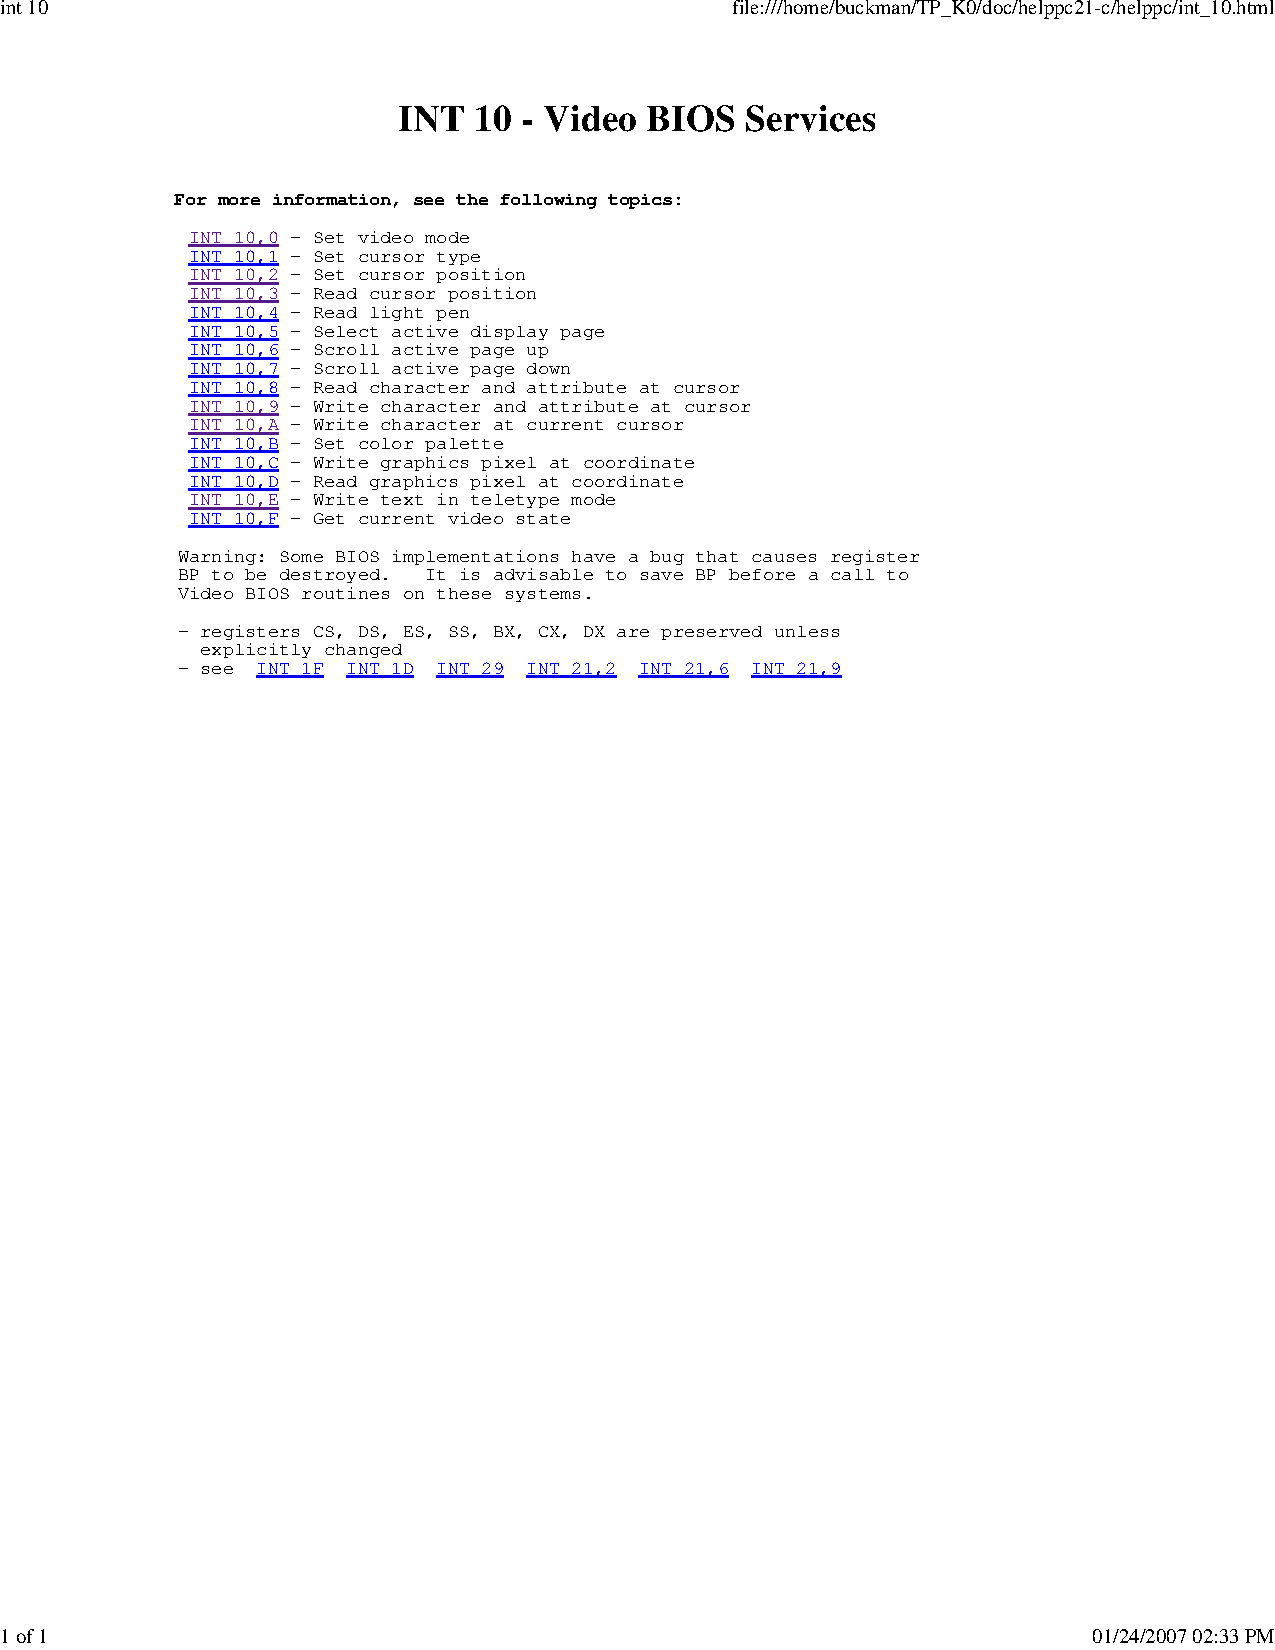
\includepdf[pages=-]{int10}
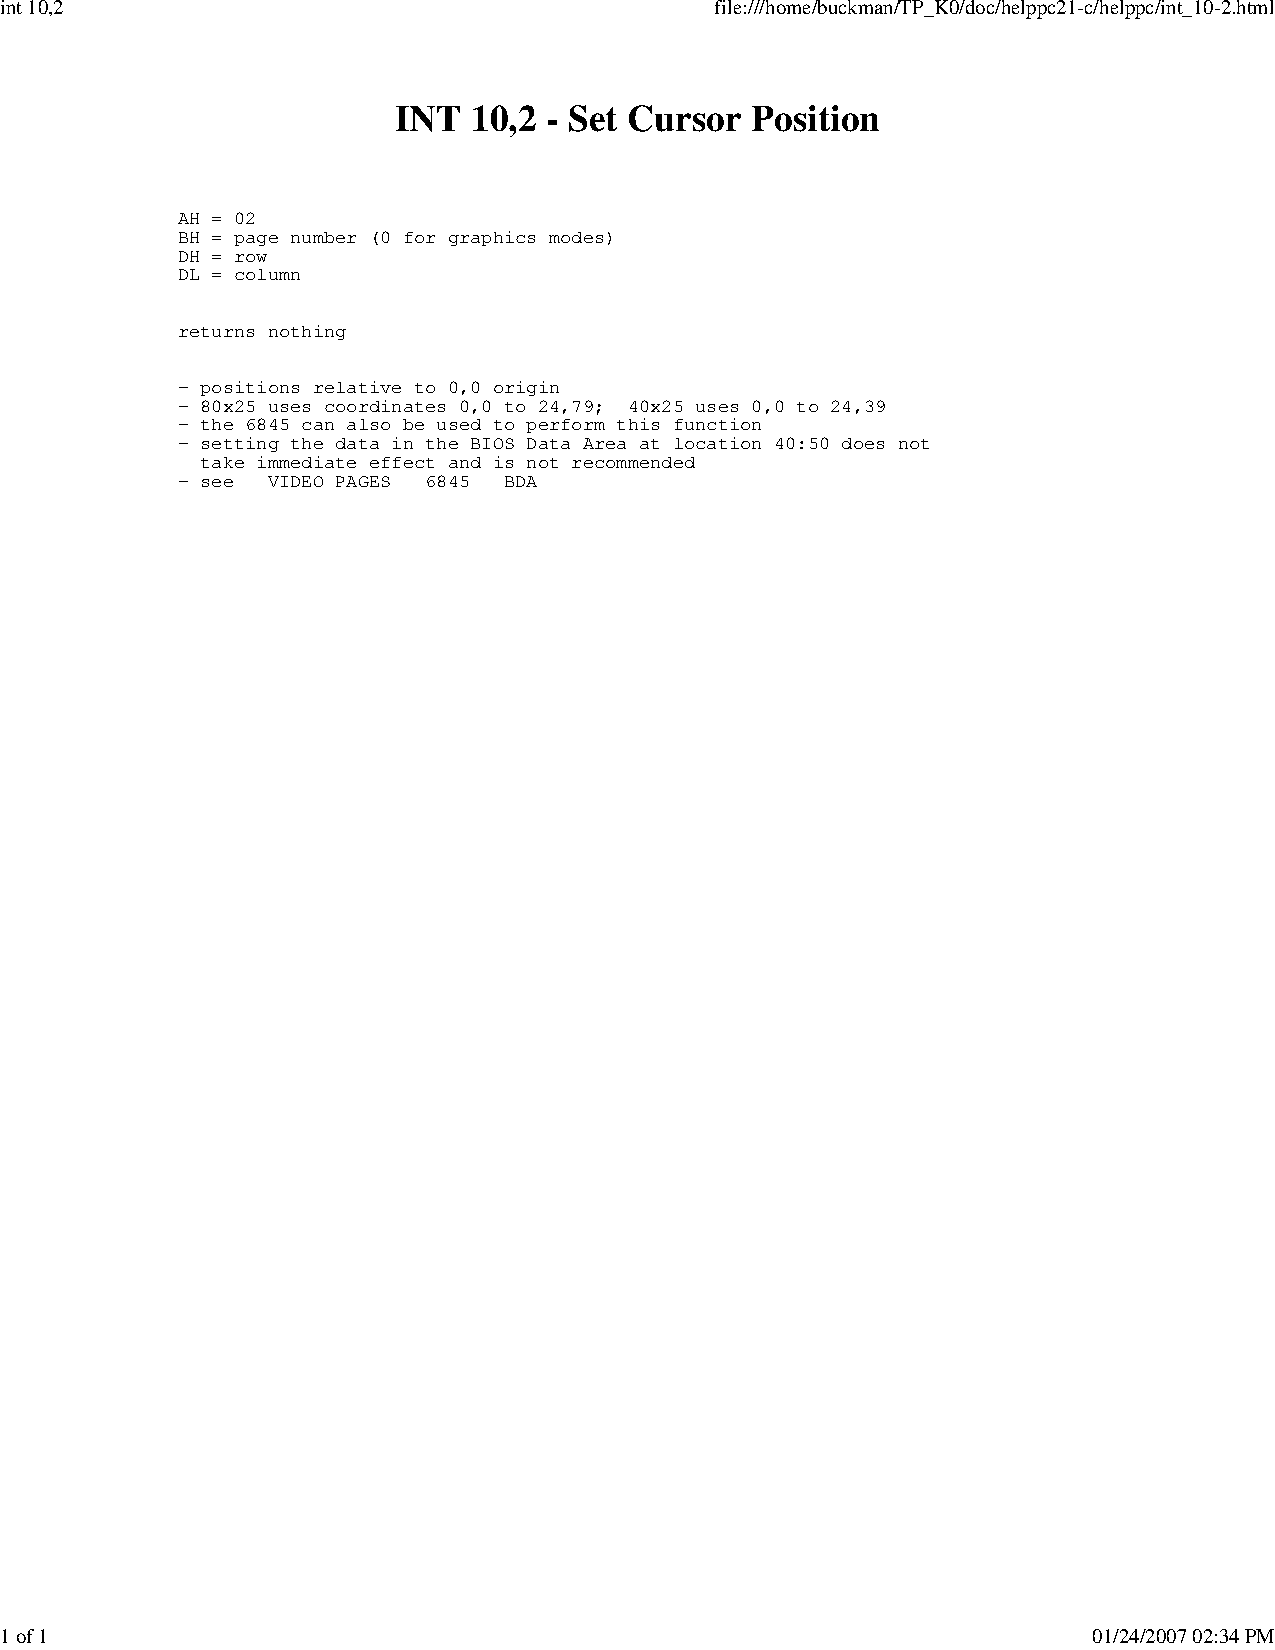
\includepdf[pages=-]{int10_2}
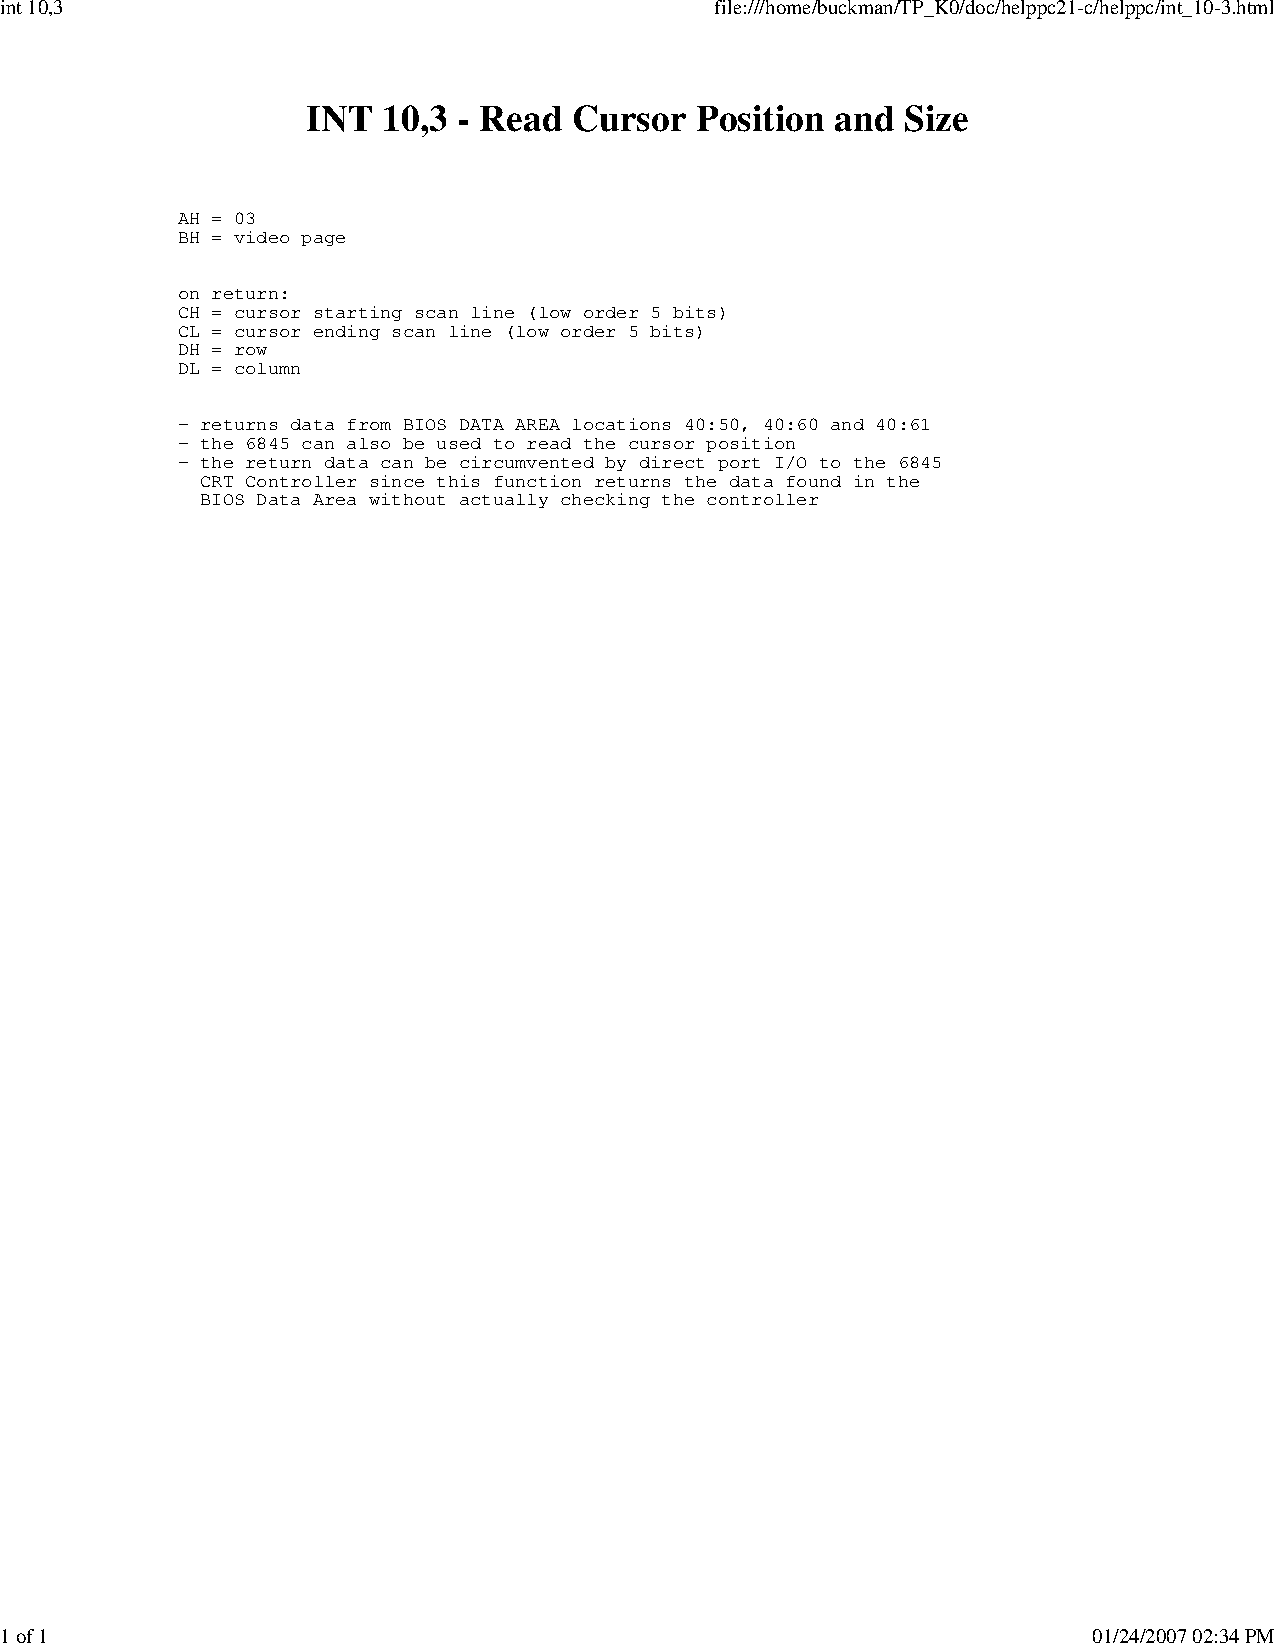
\includepdf[pages=-]{int10_3}
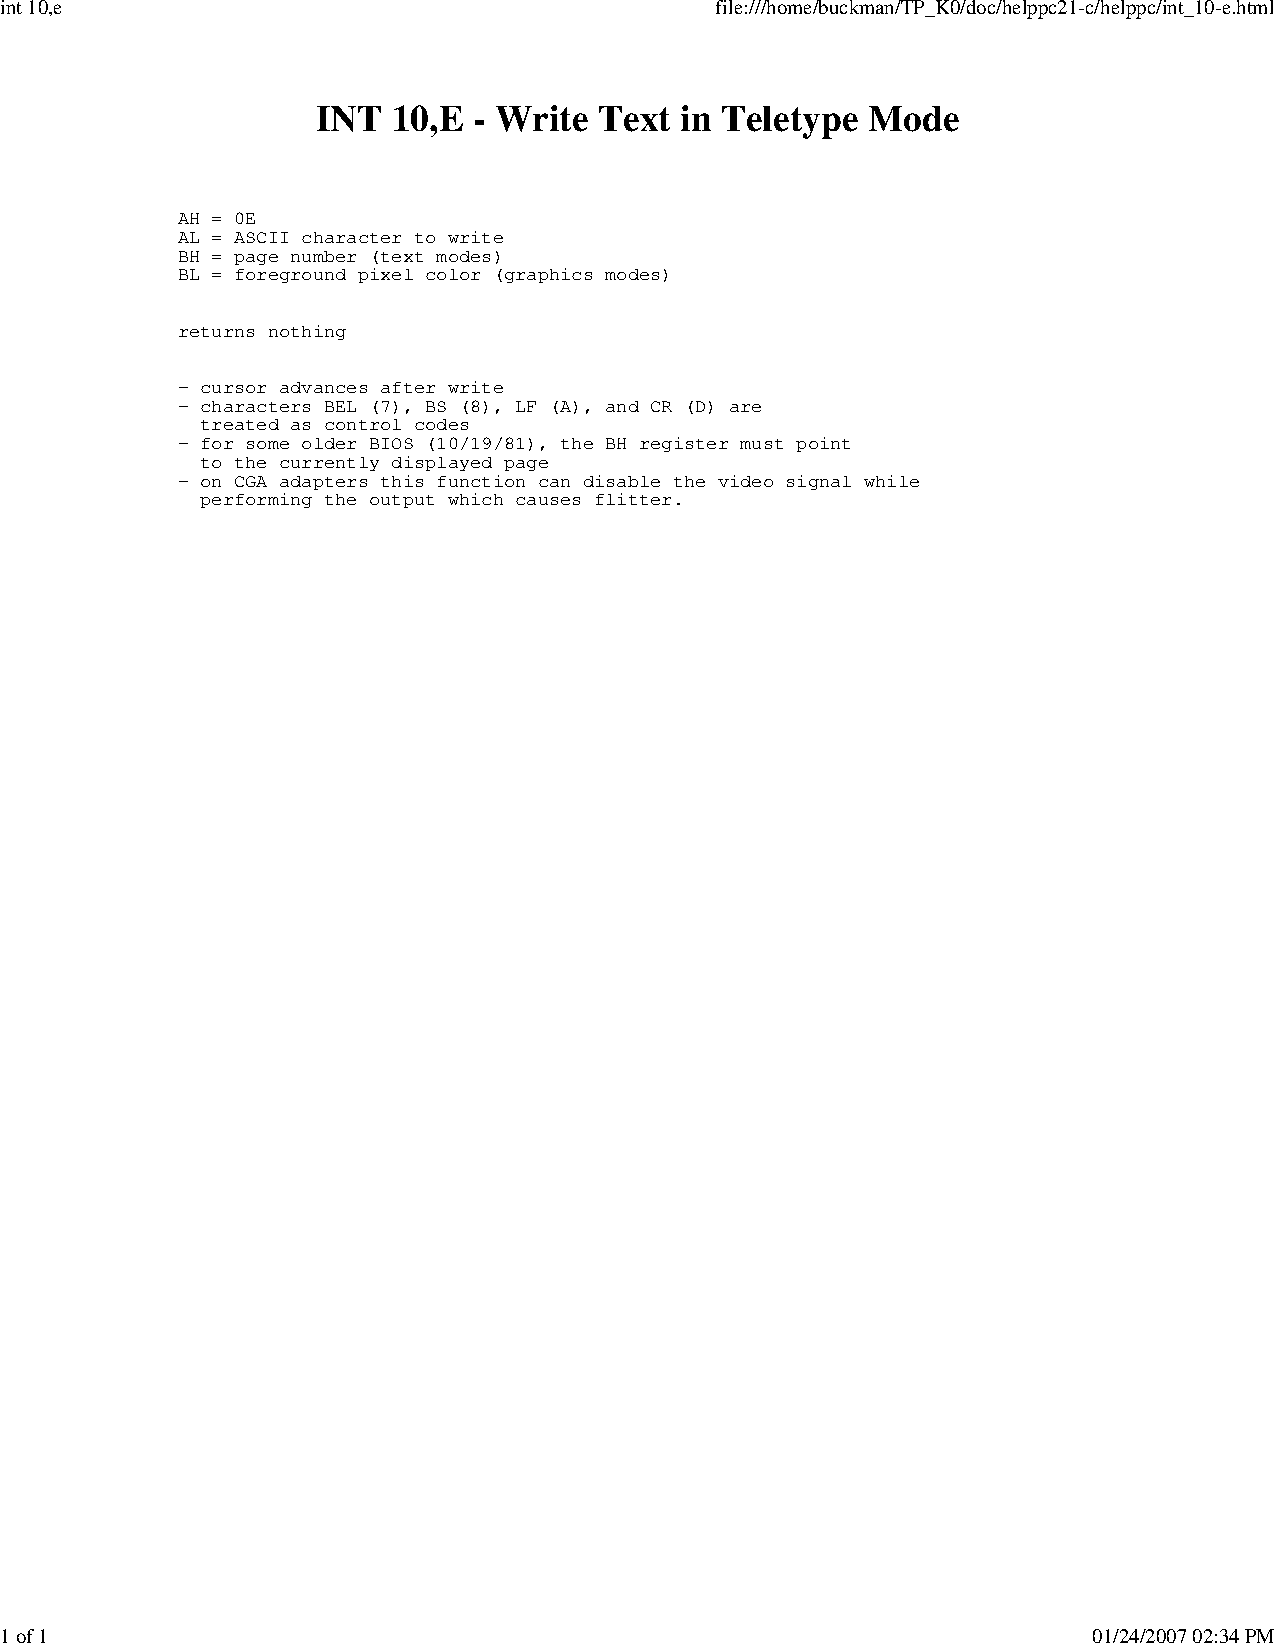
\includepdf[pages=-]{int10_e}

\subsection{Disks accesses}
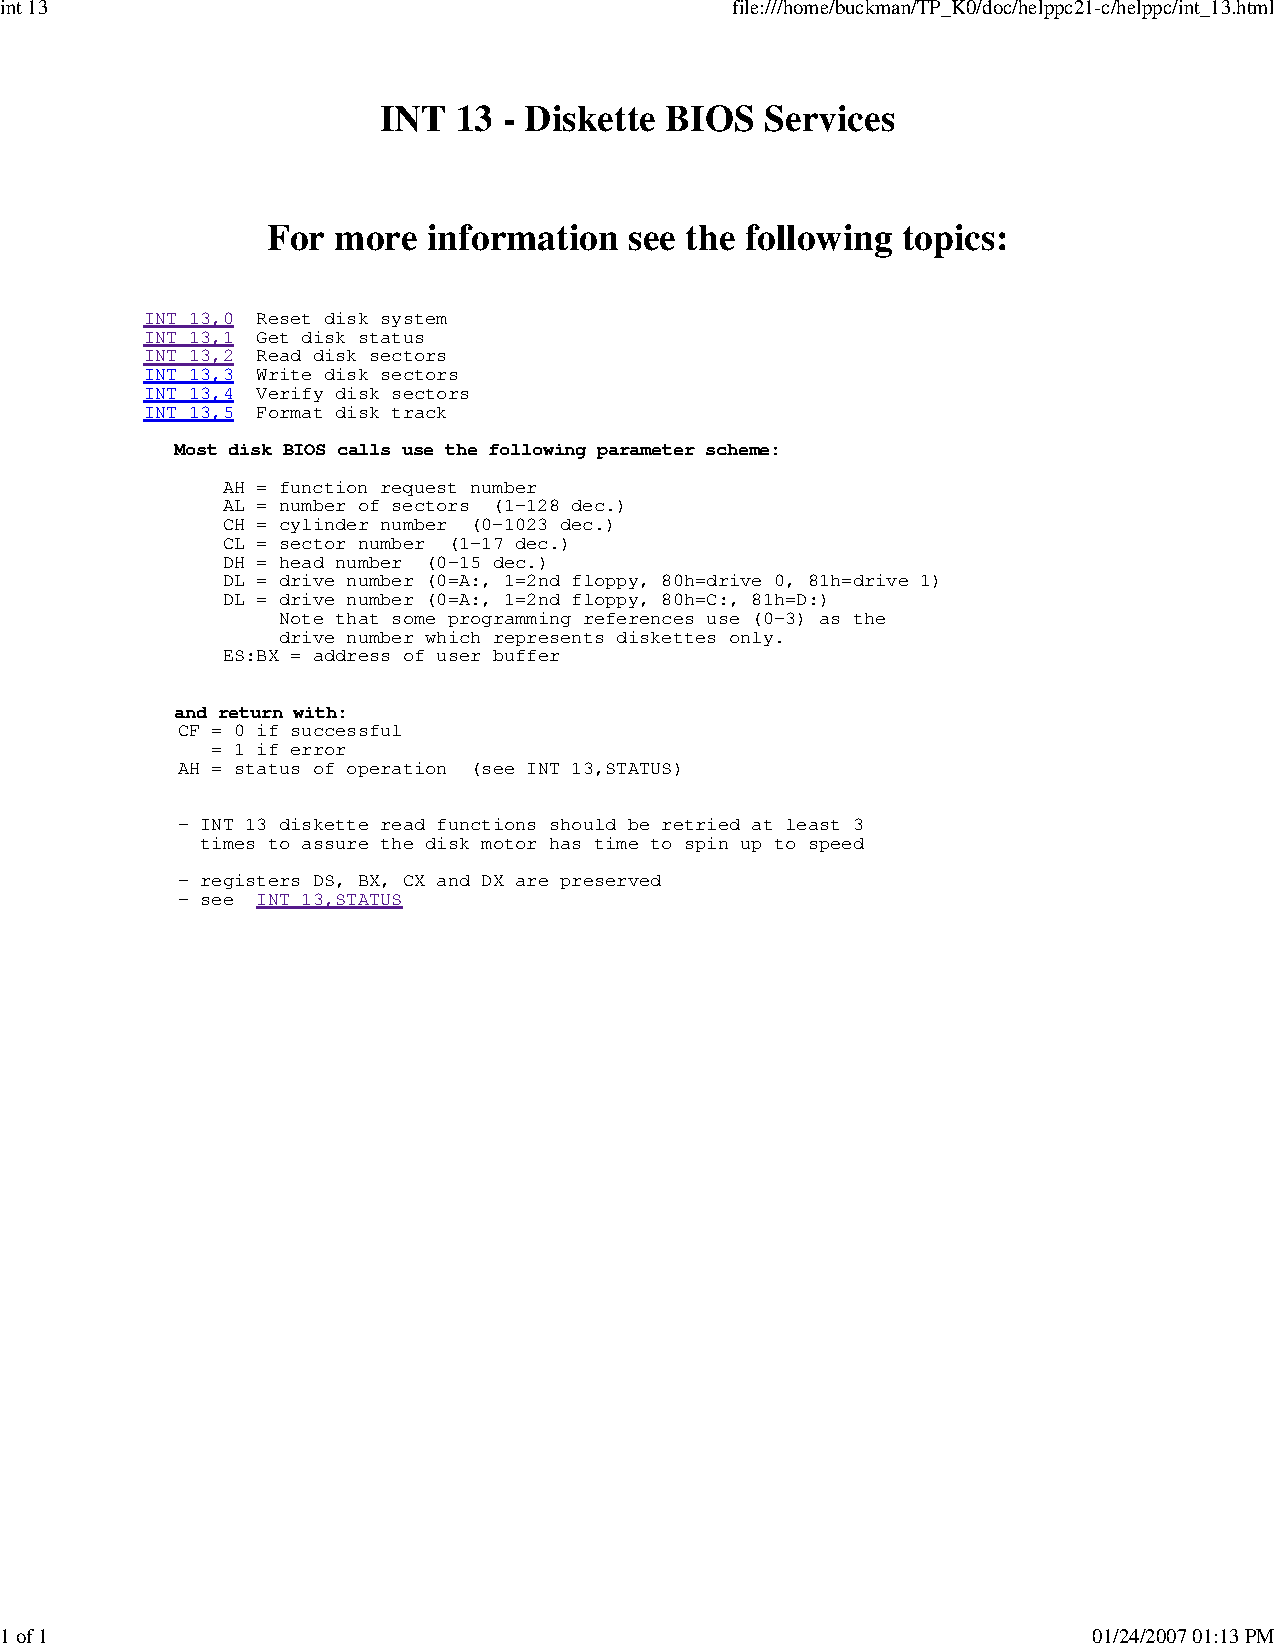
\includepdf[pages=-]{int13}
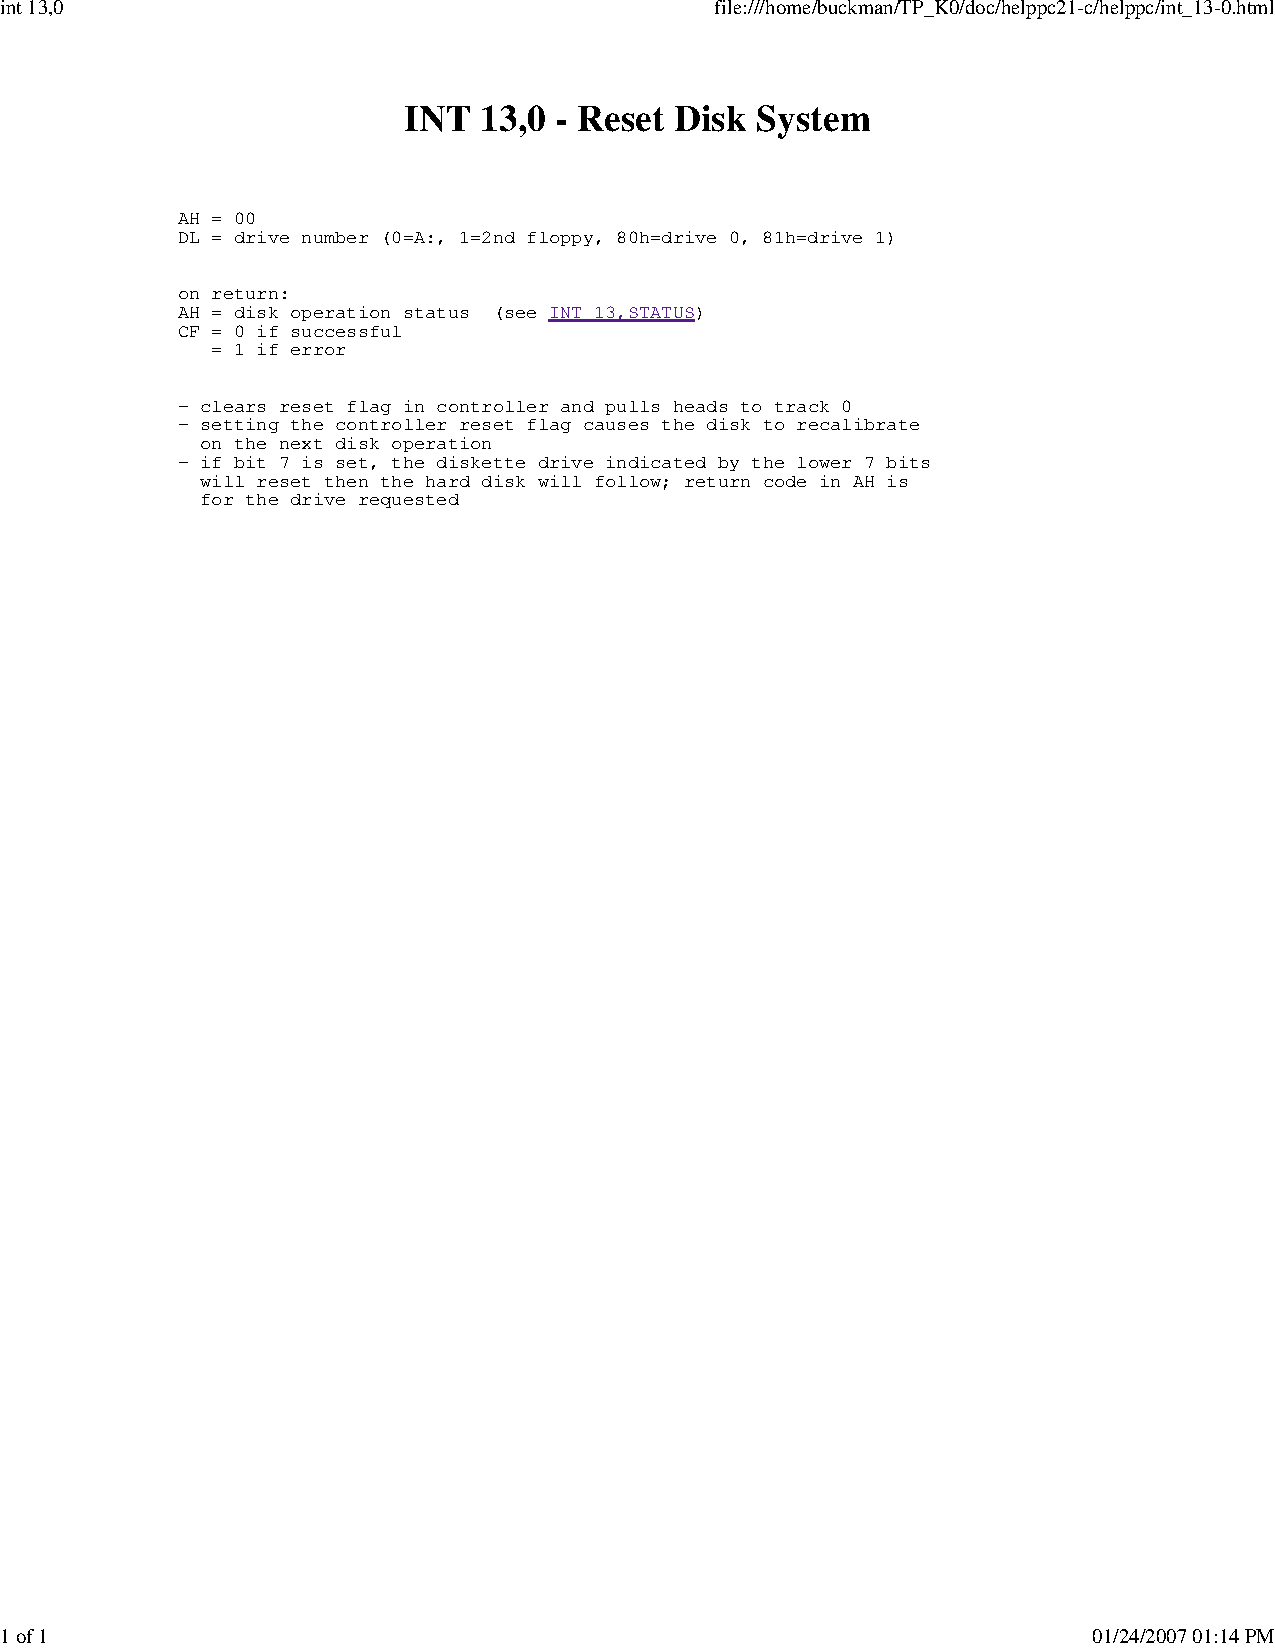
\includepdf[pages=-]{int13_0}
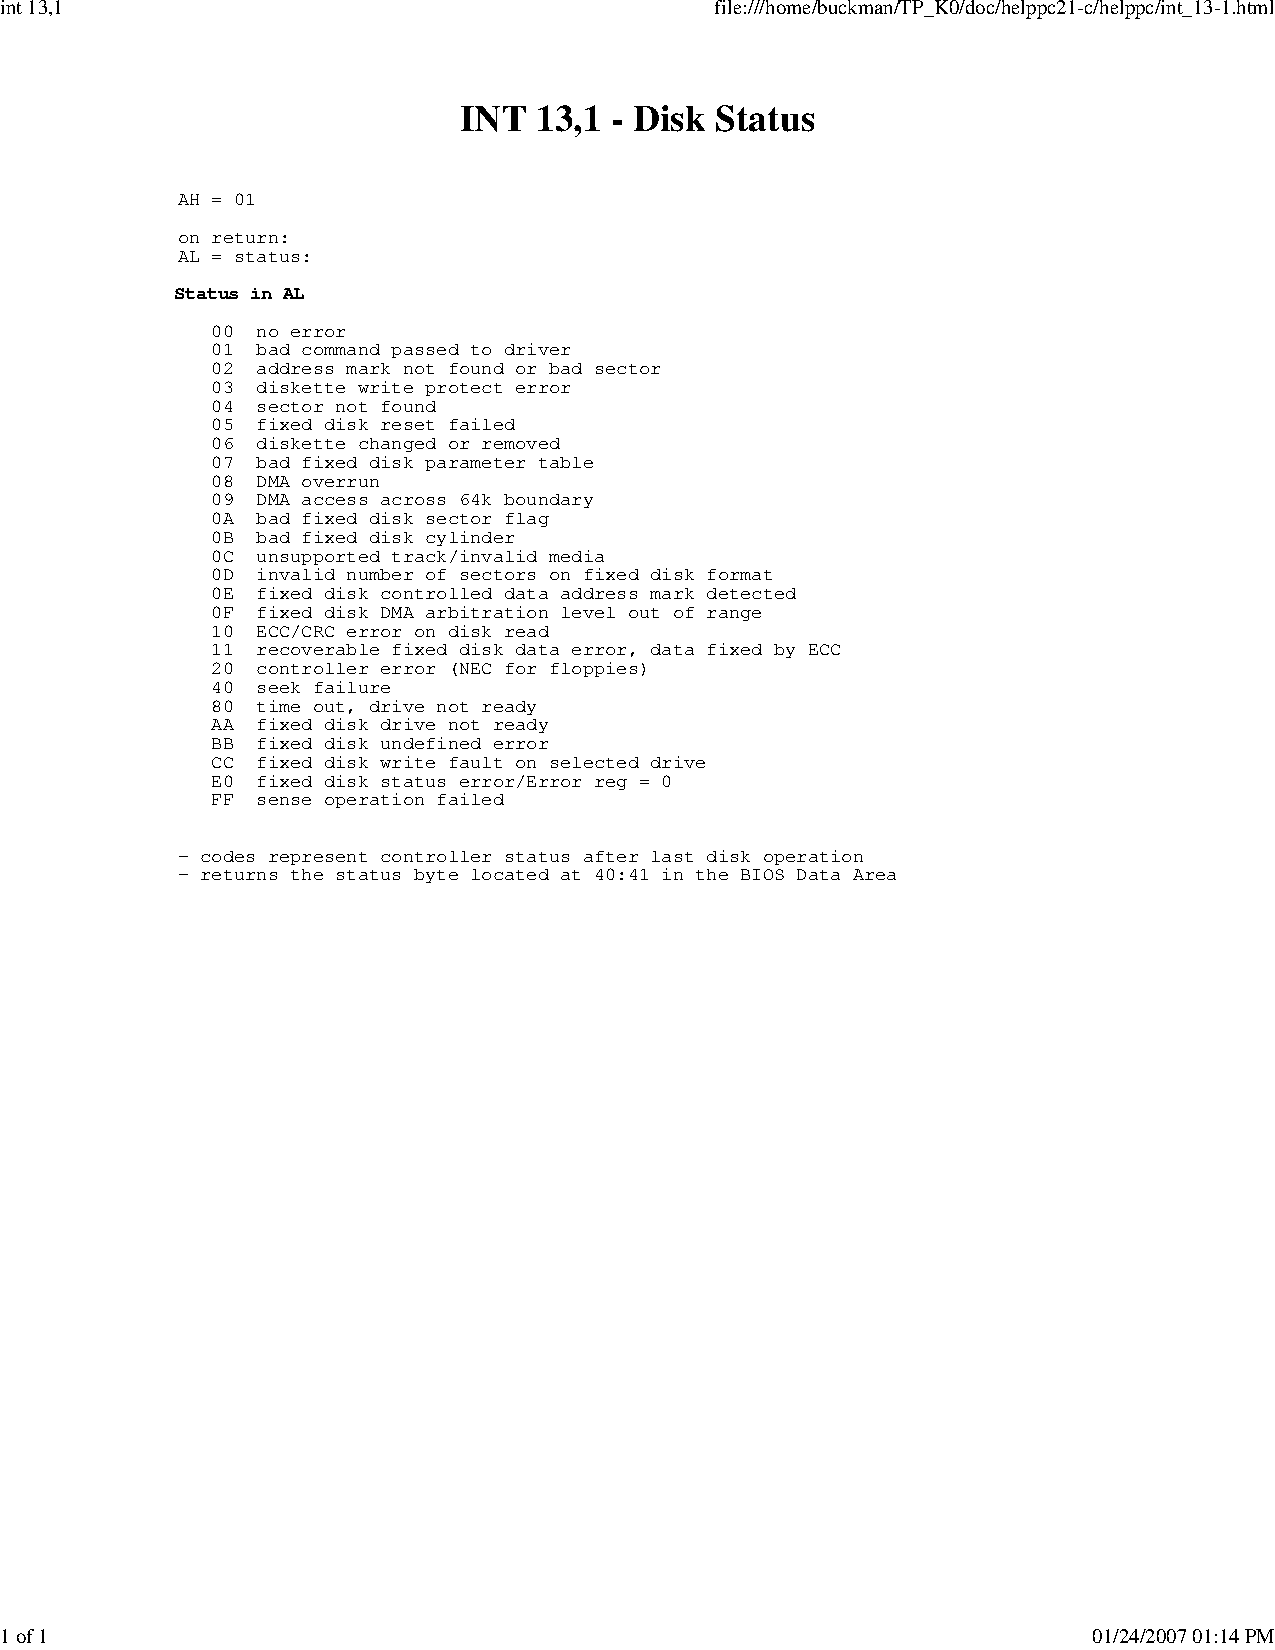
\includepdf[pages=-]{int13_1}
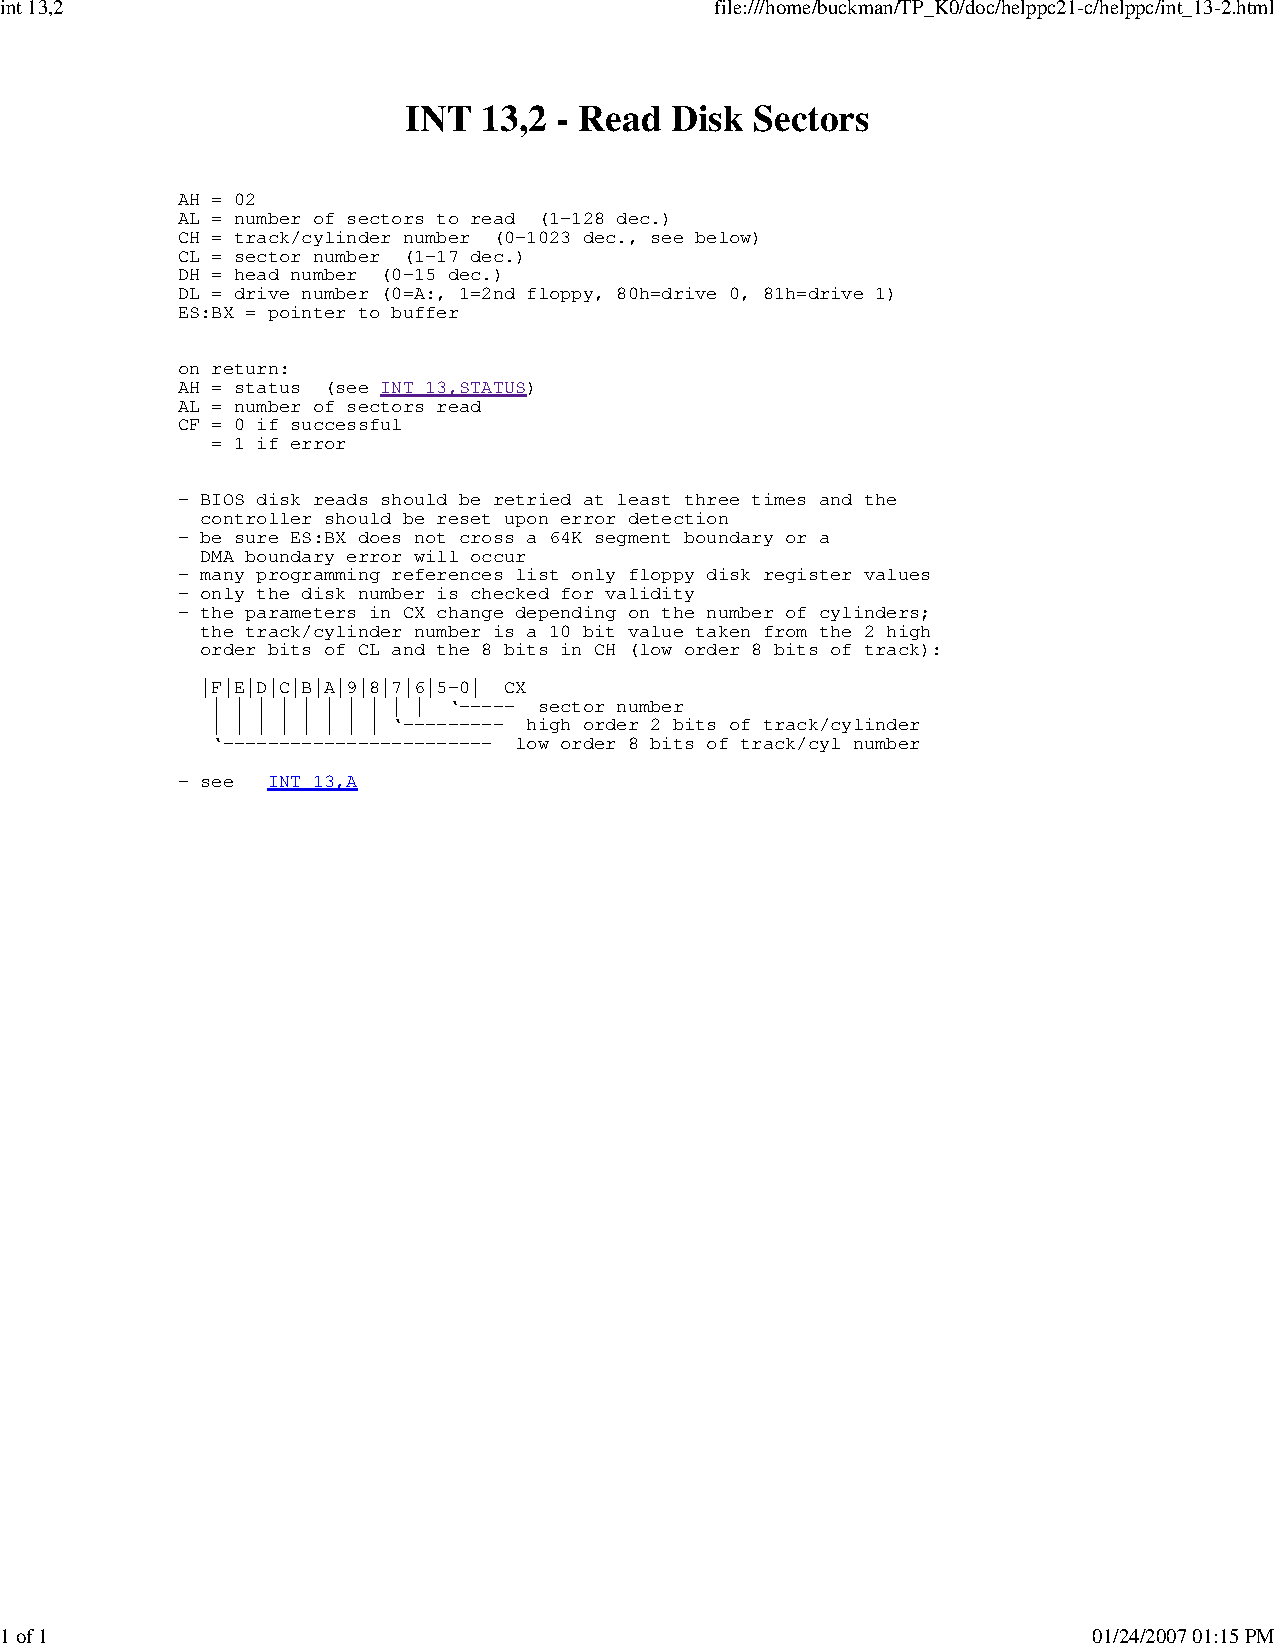
\includepdf[pages=-]{int13_2}

\subsection{Keyboard}
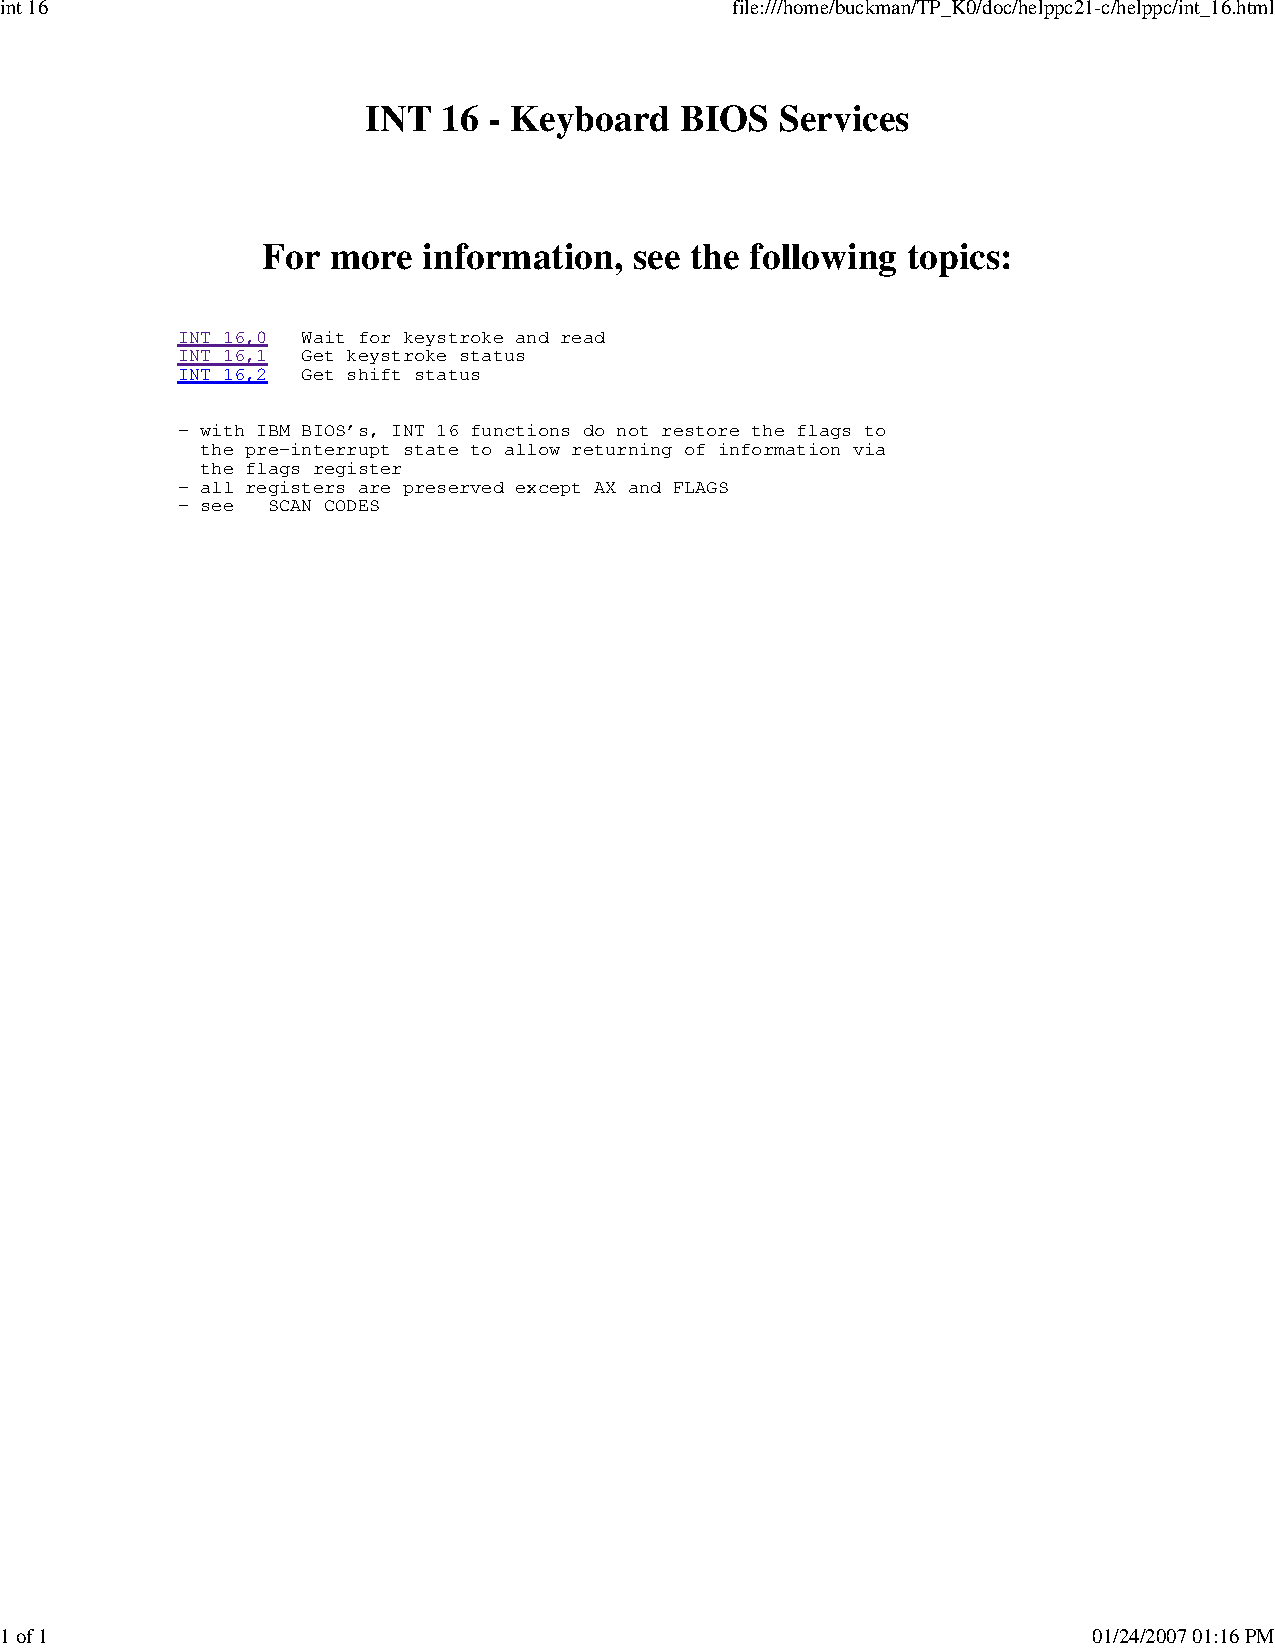
\includepdf[pages=-]{int16}
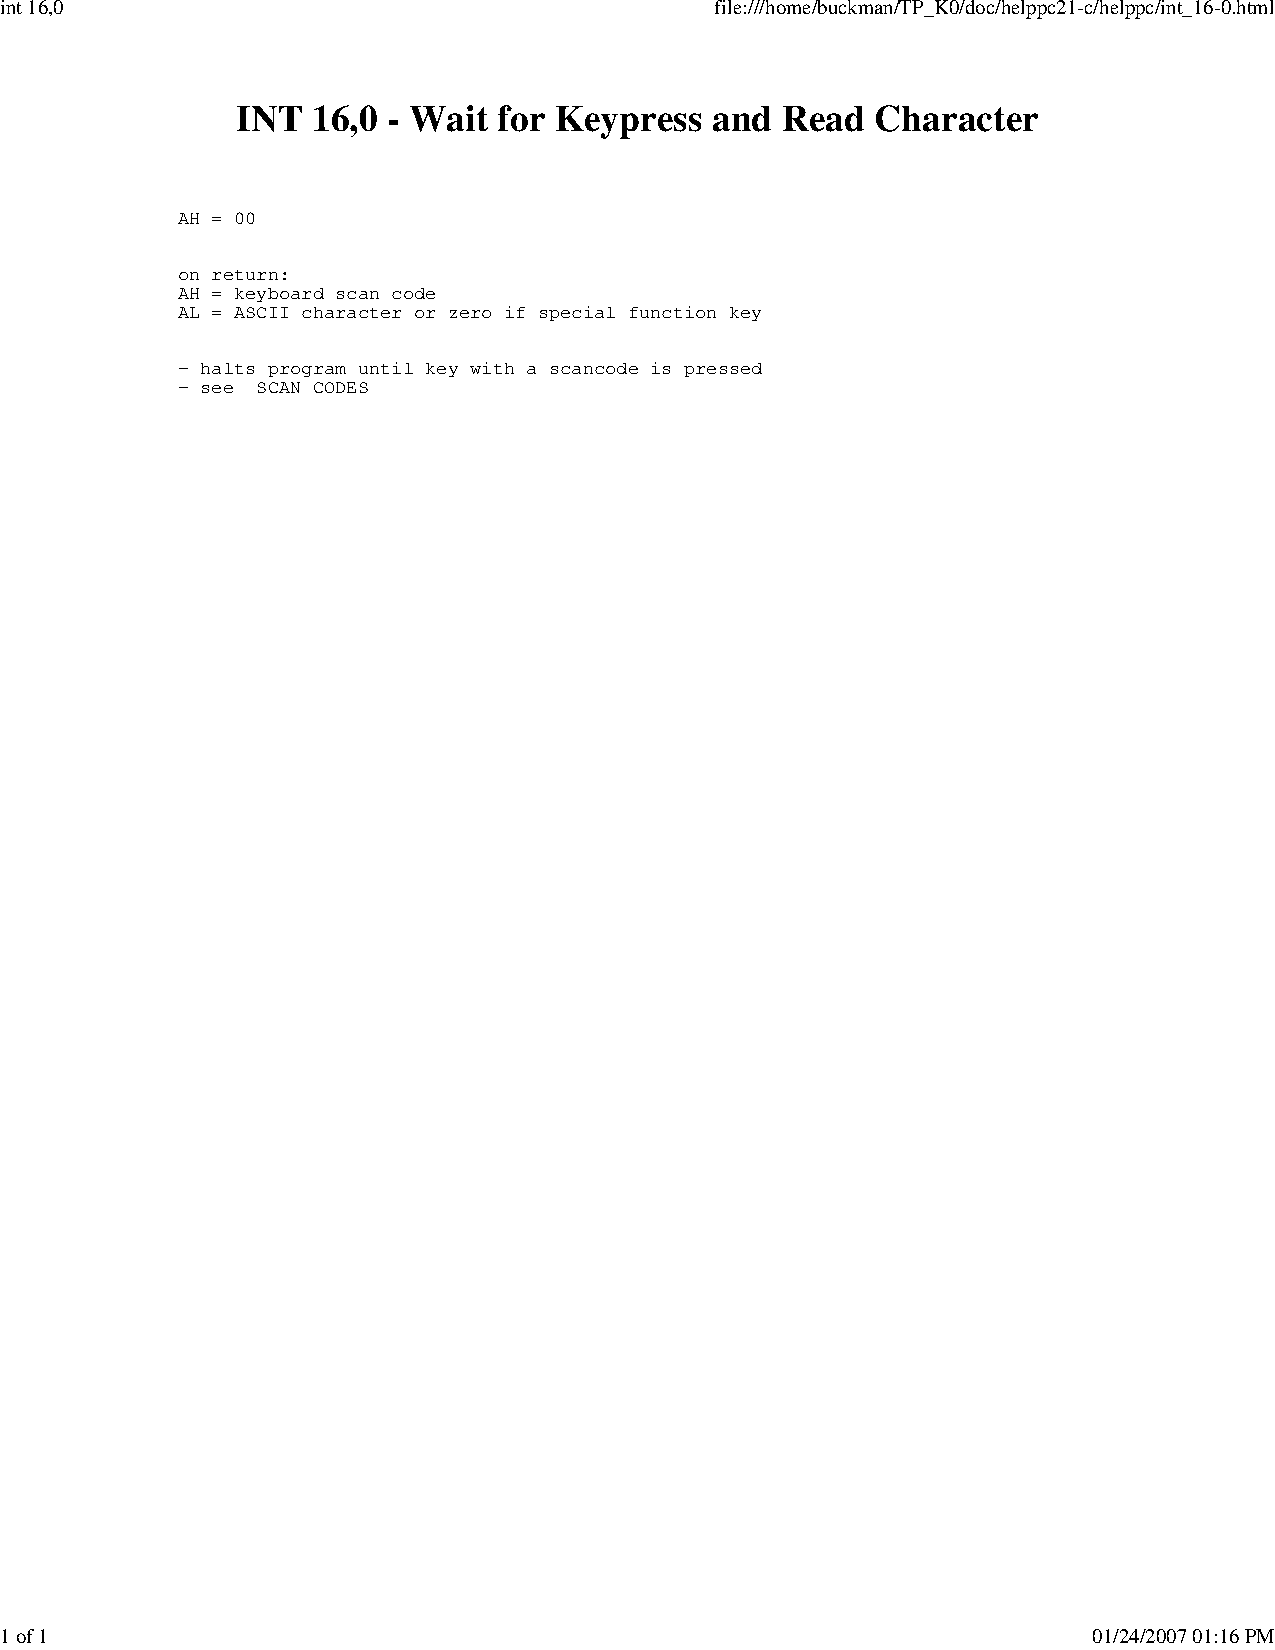
\includepdf[pages=-]{int16_0}
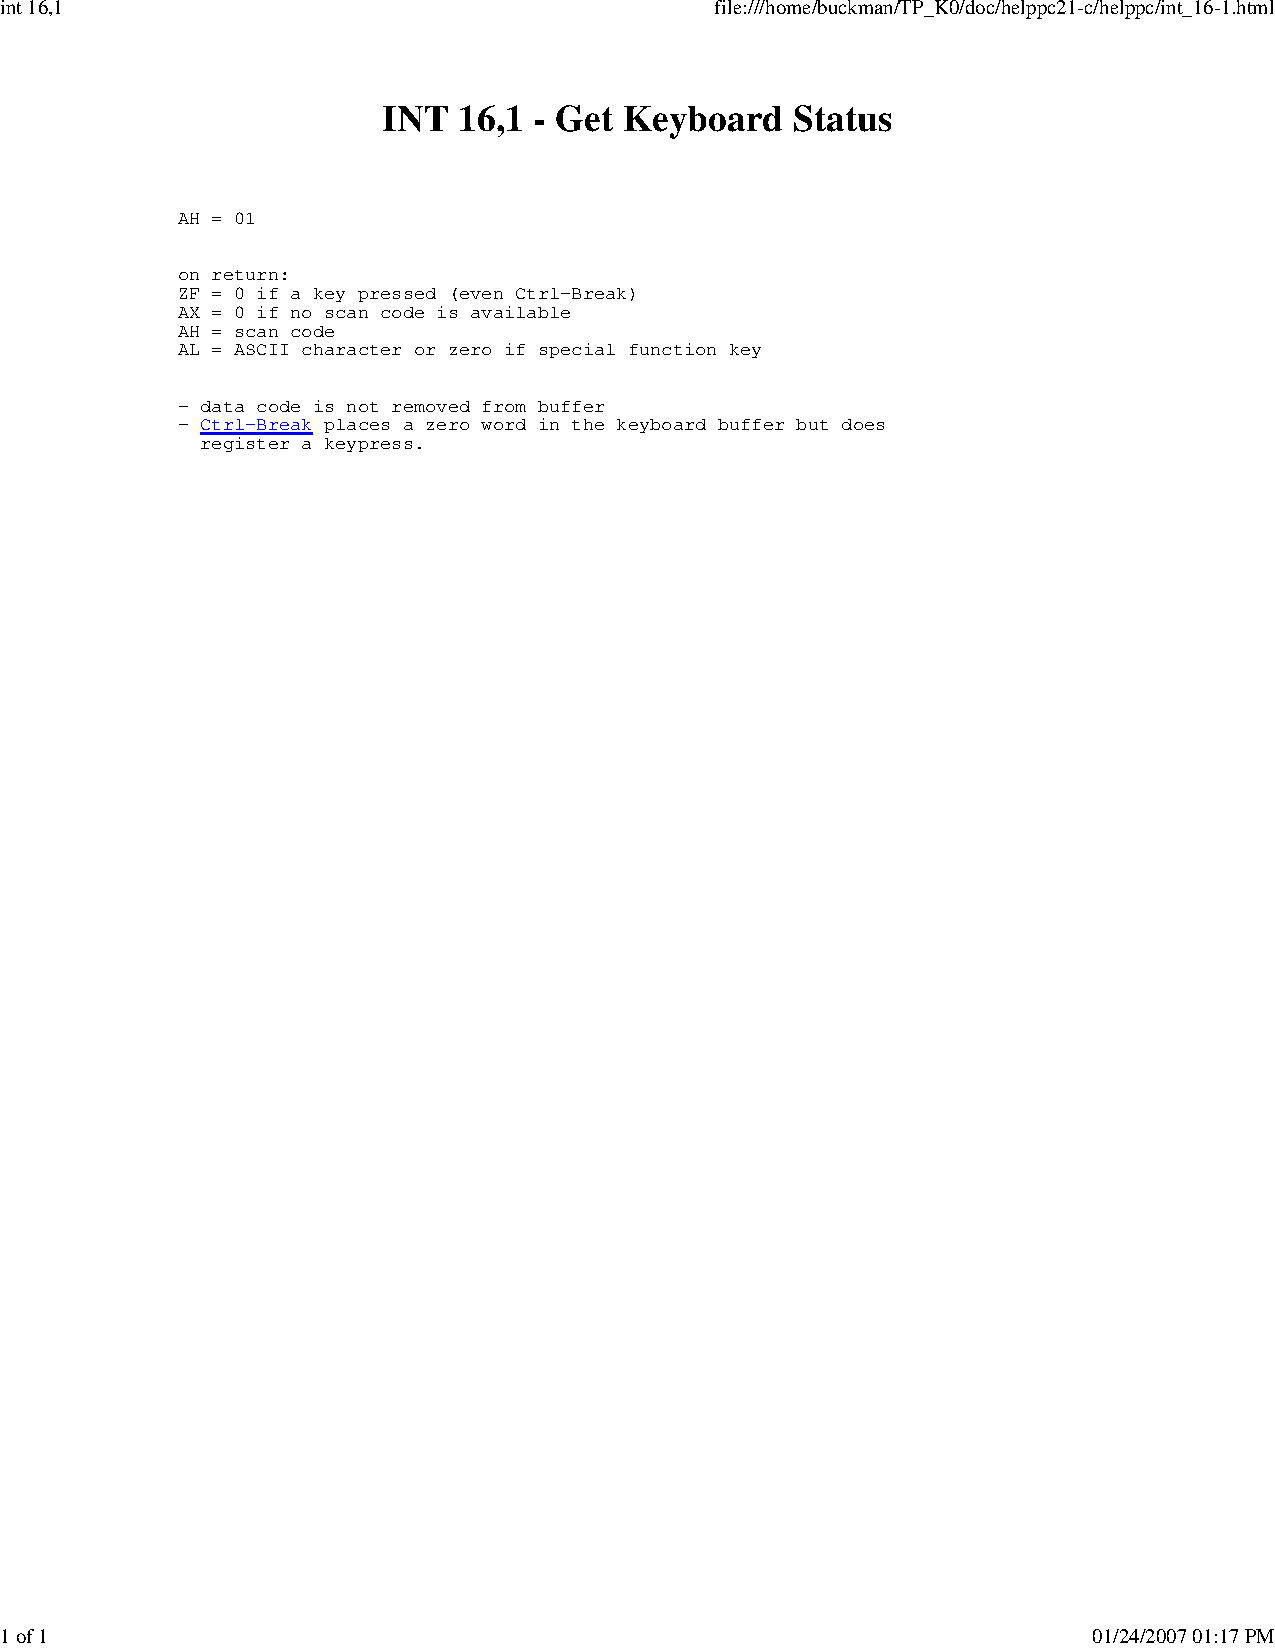
\includepdf[pages=-]{int16_1}
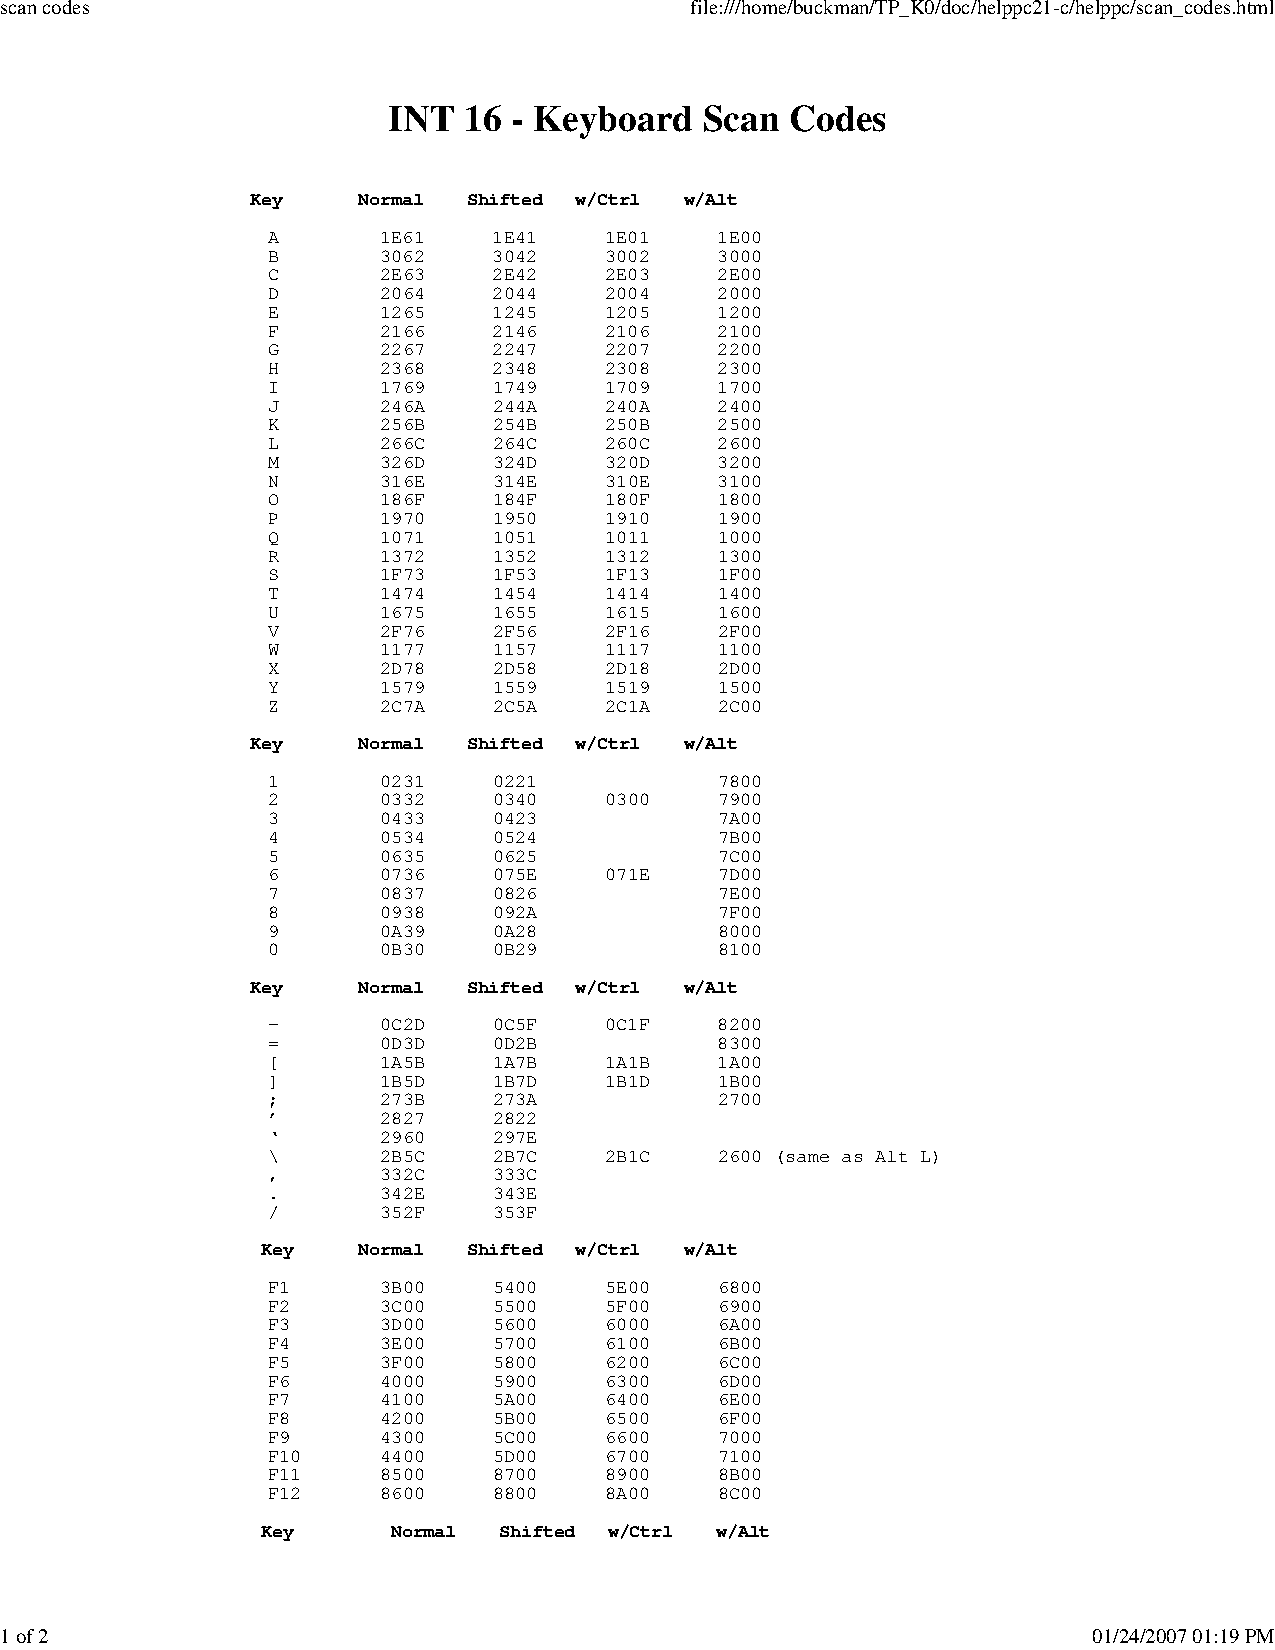
\includepdf[pages=-]{int16_scancodes}

%
% ELF documentation
%

\section{ELF format}

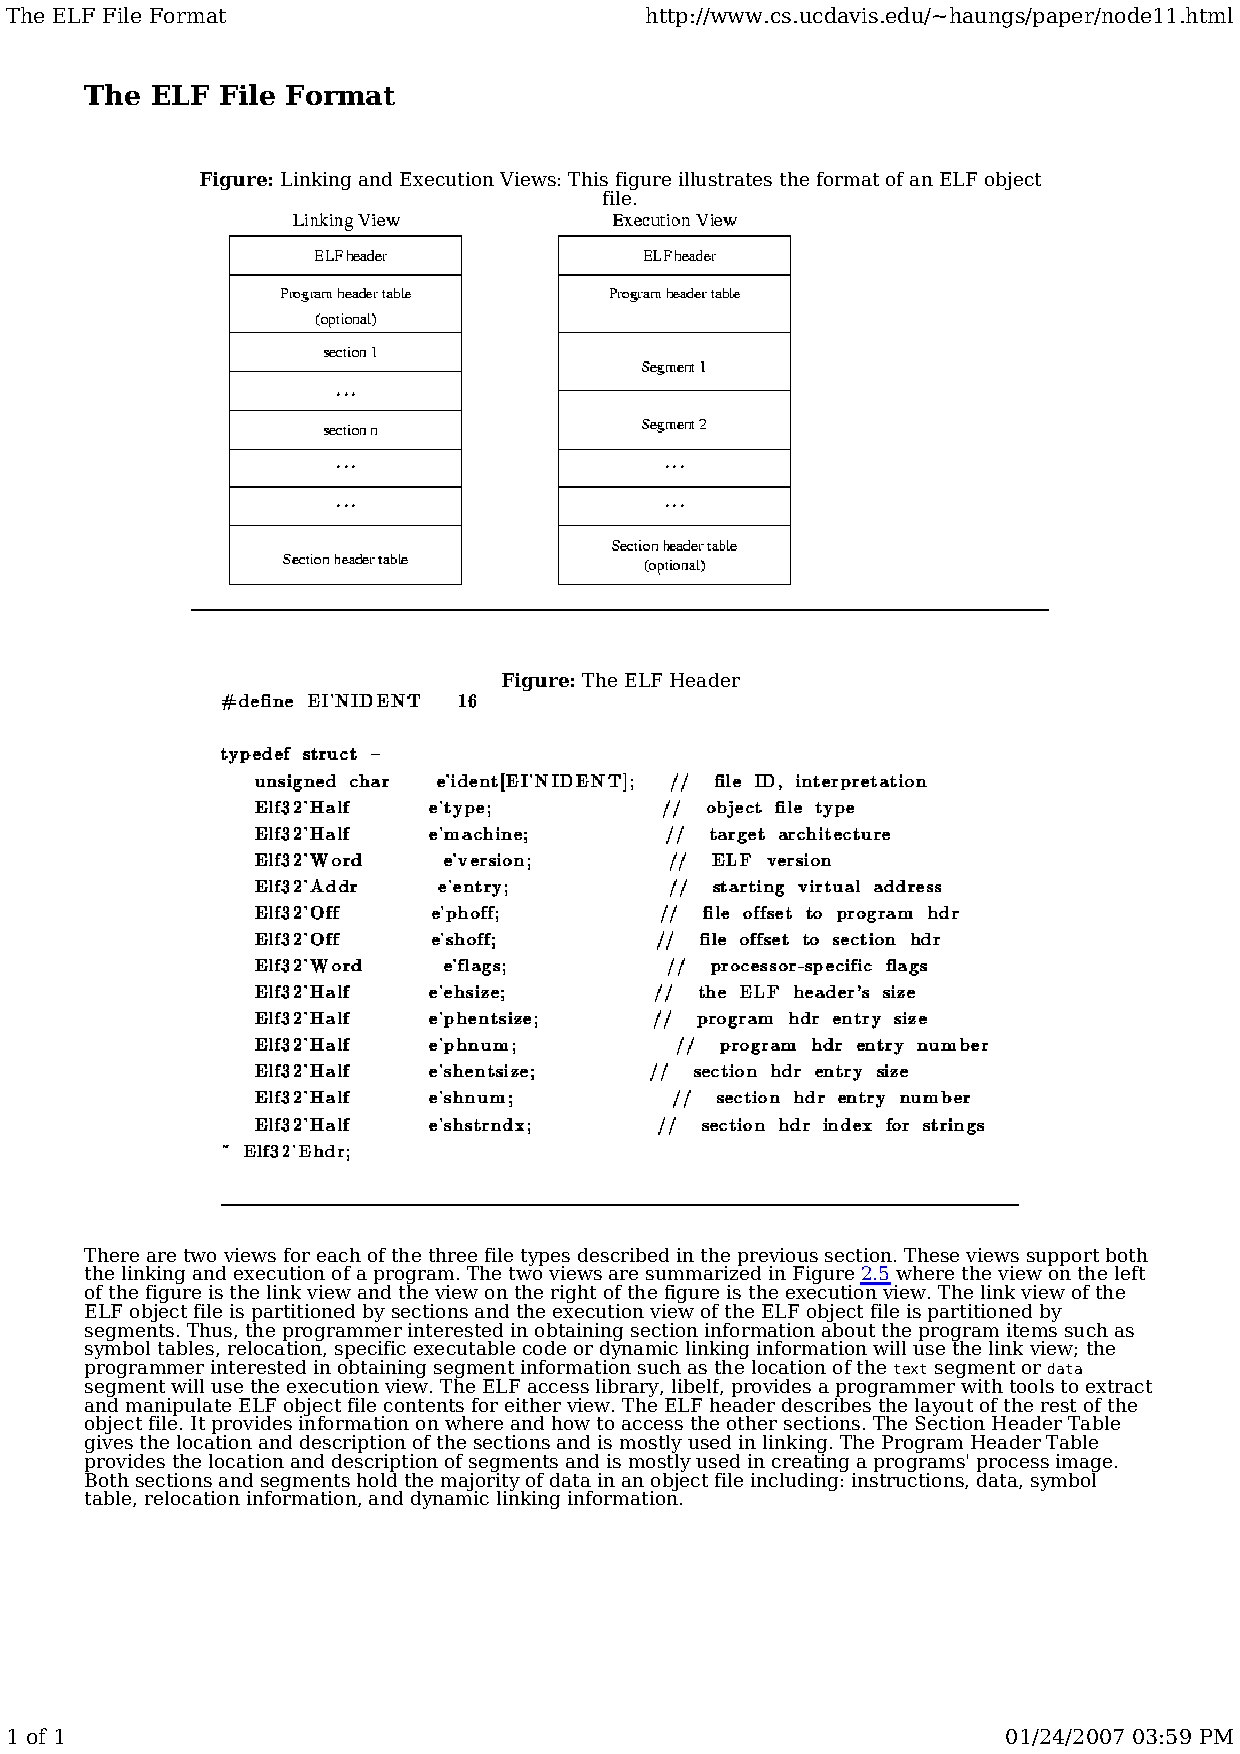
\includepdf[pages=-]{elf1}
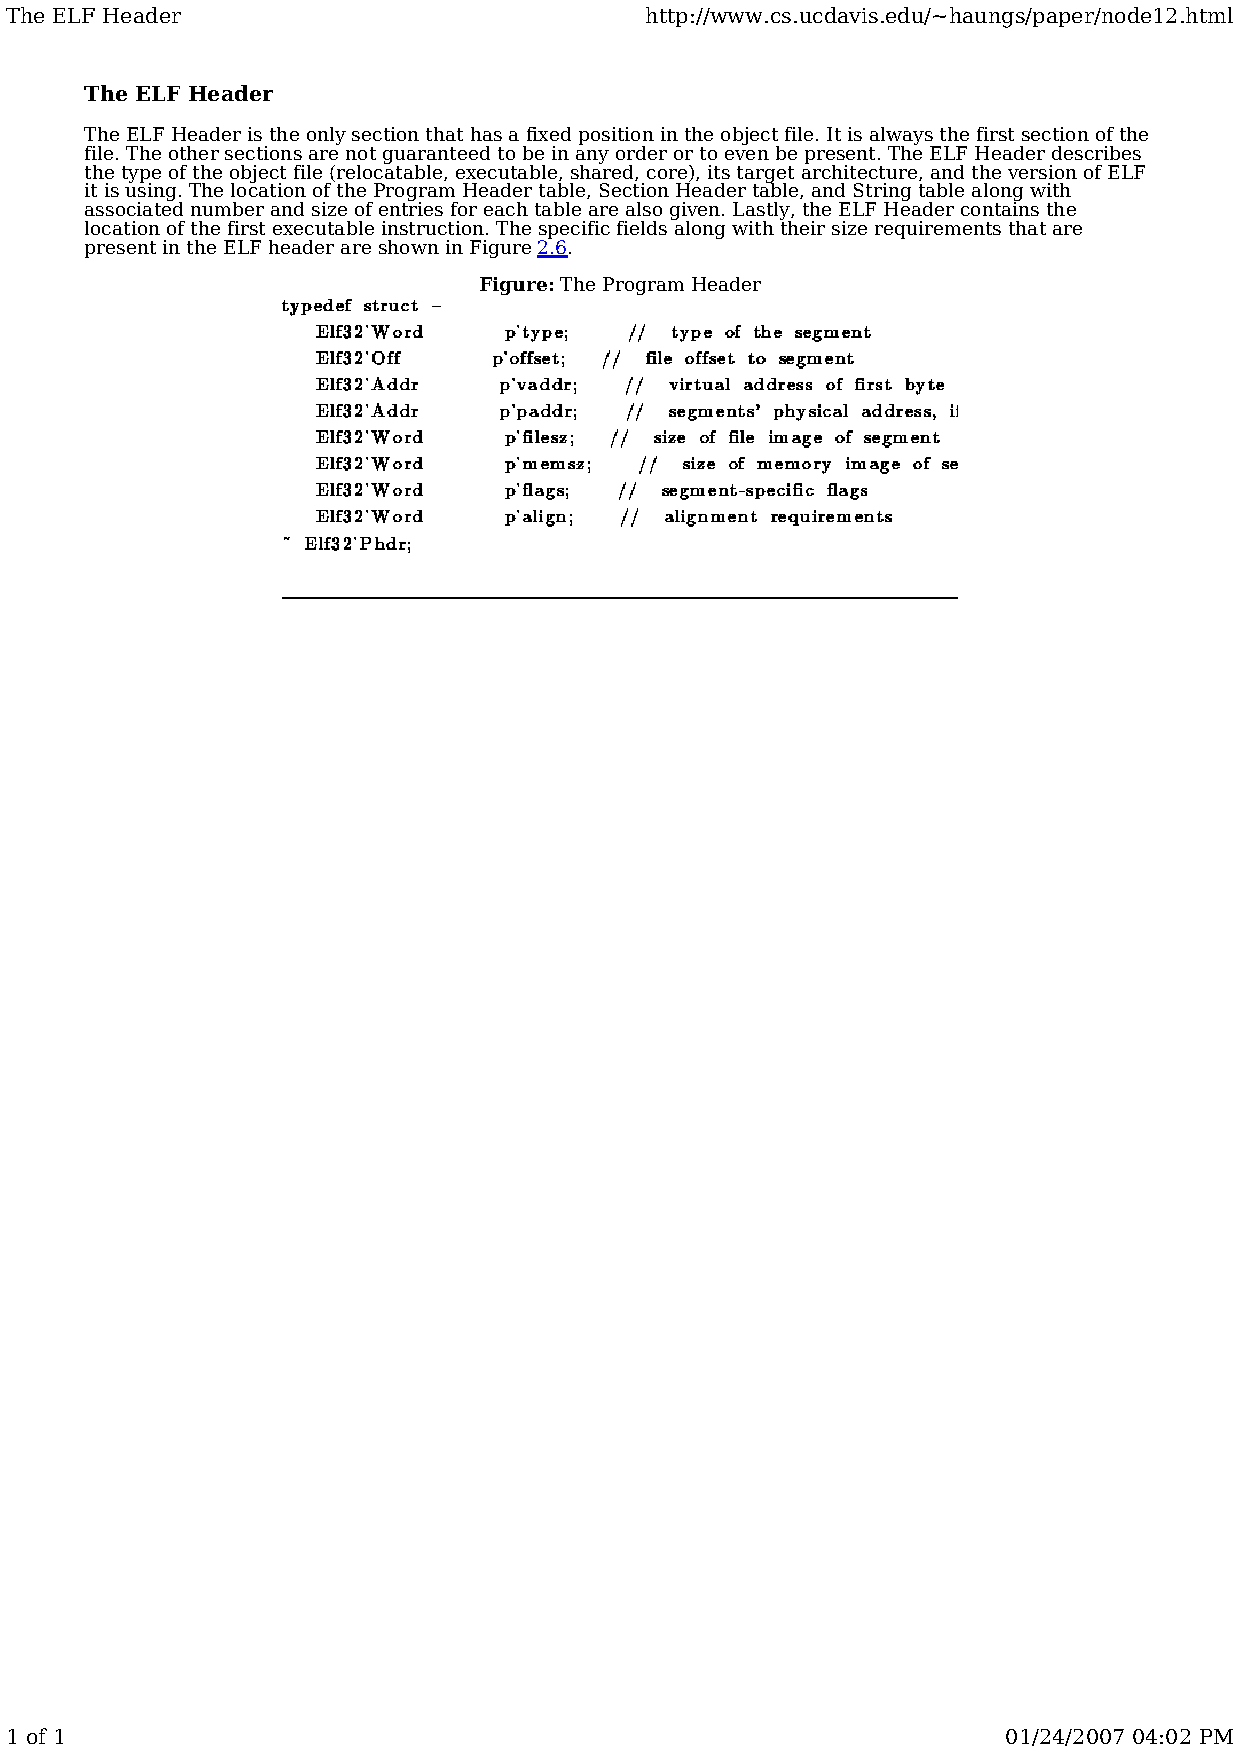
\includepdf[pages=-]{elf2}
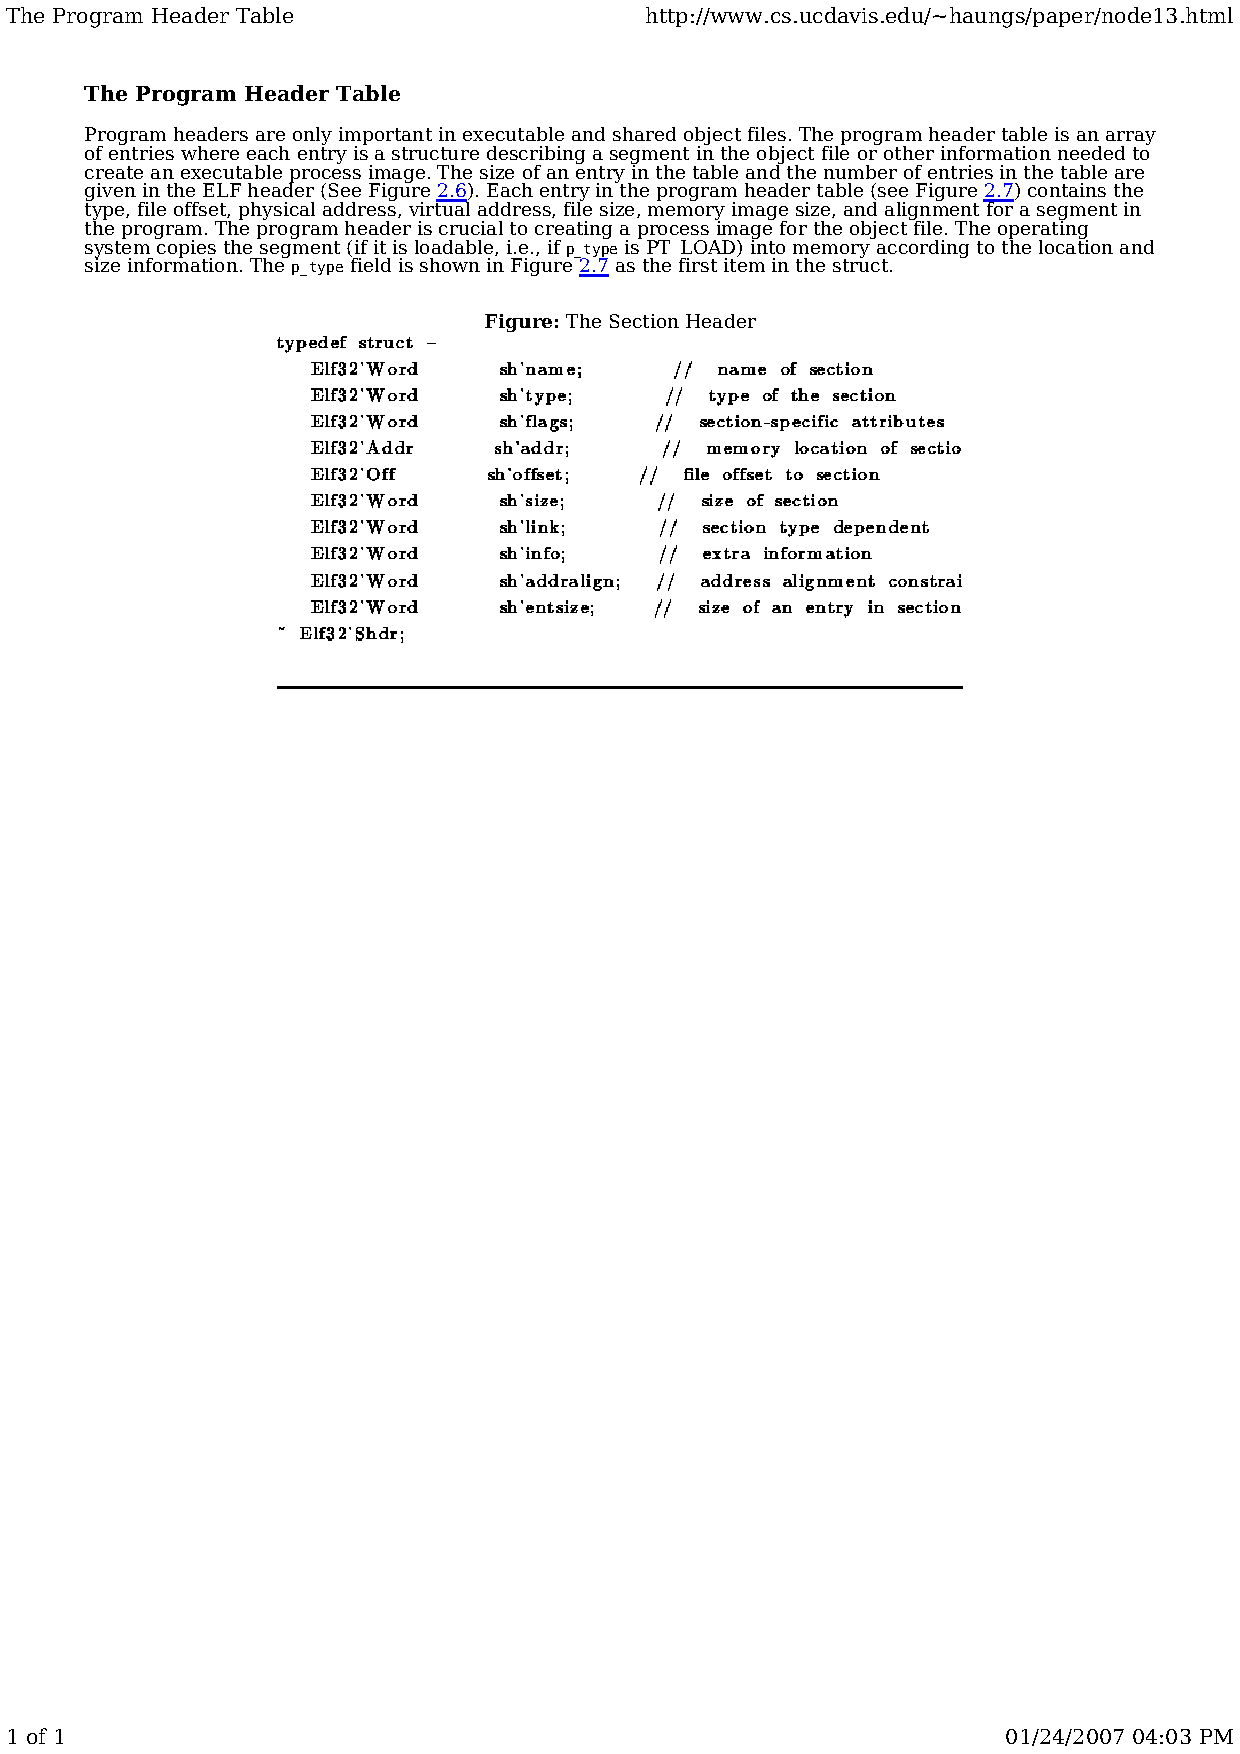
\includepdf[pages=-]{elf3}
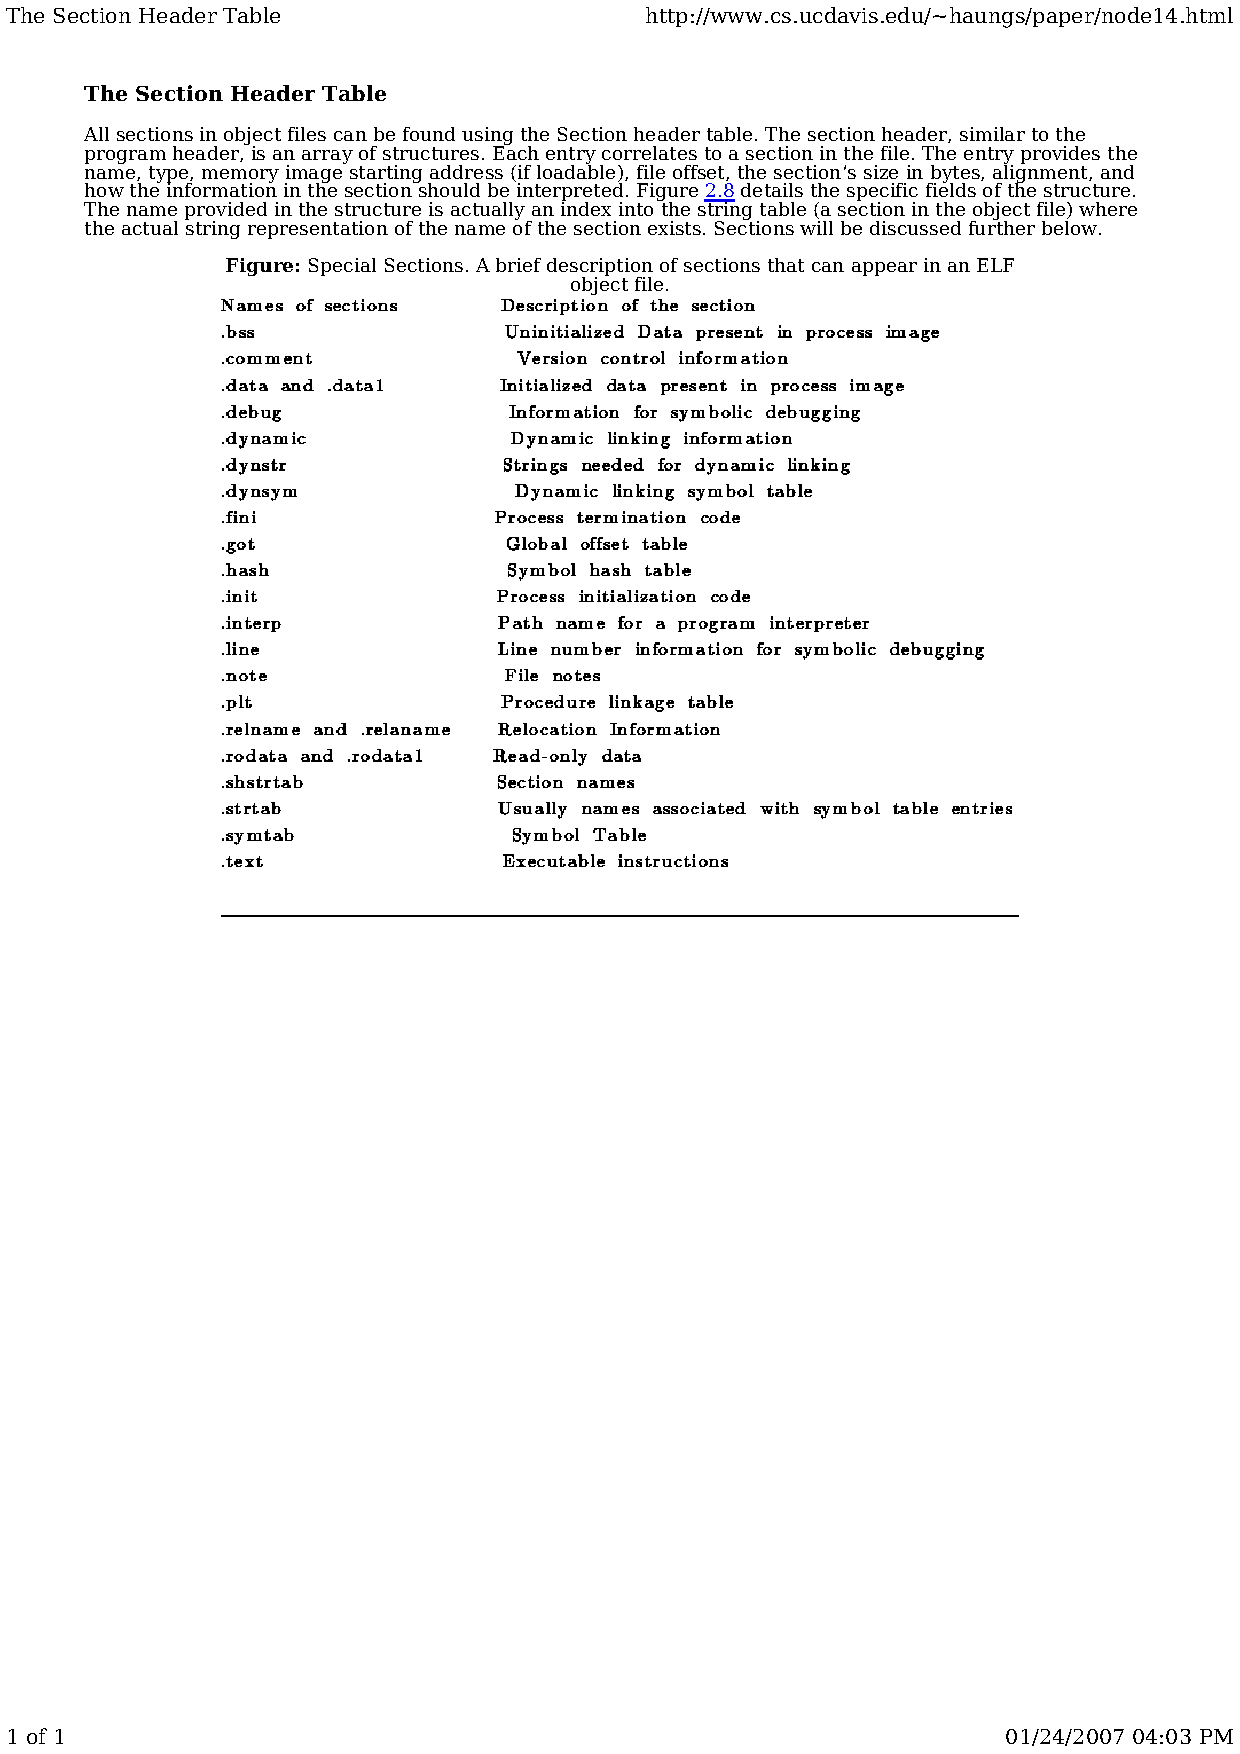
\includepdf[pages=-]{elf4}
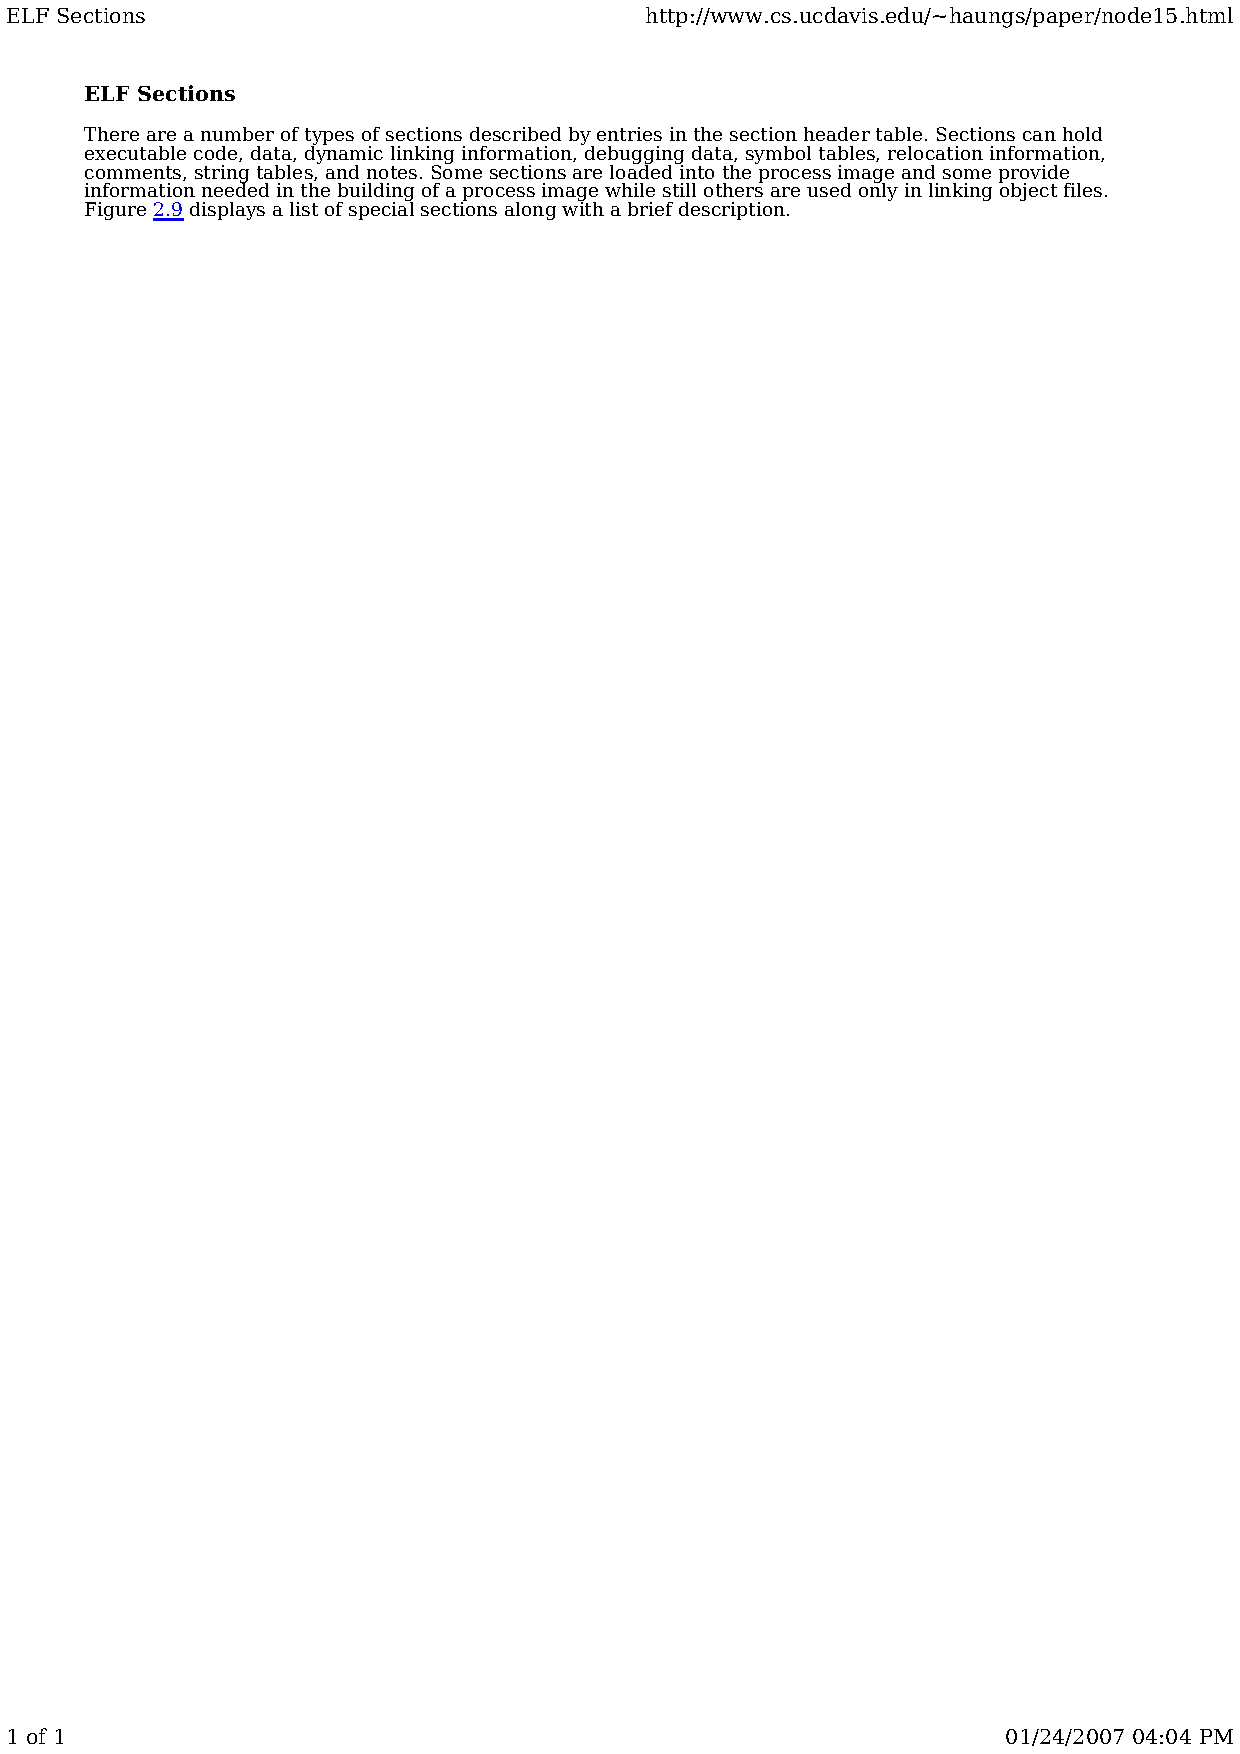
\includepdf[pages=-]{elf5}
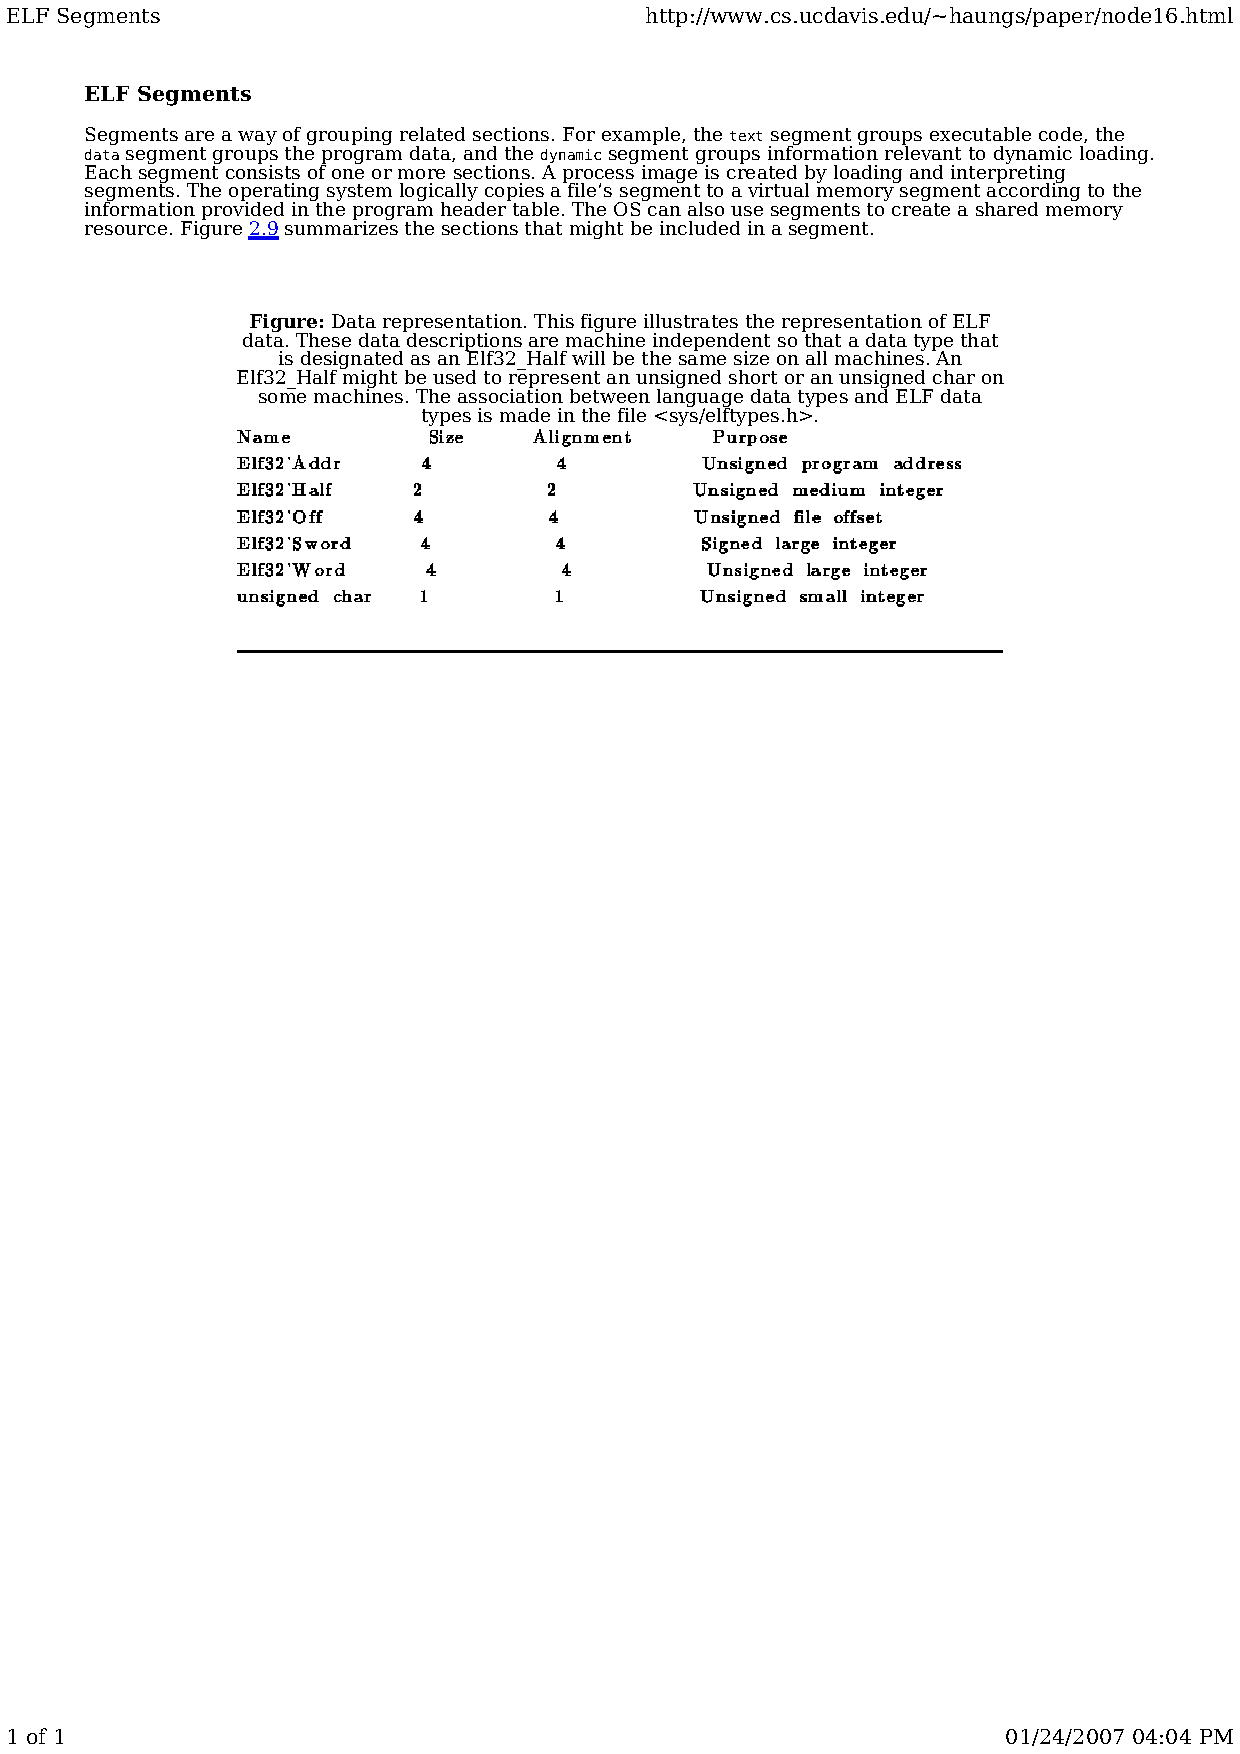
\includepdf[pages=-]{elf6}
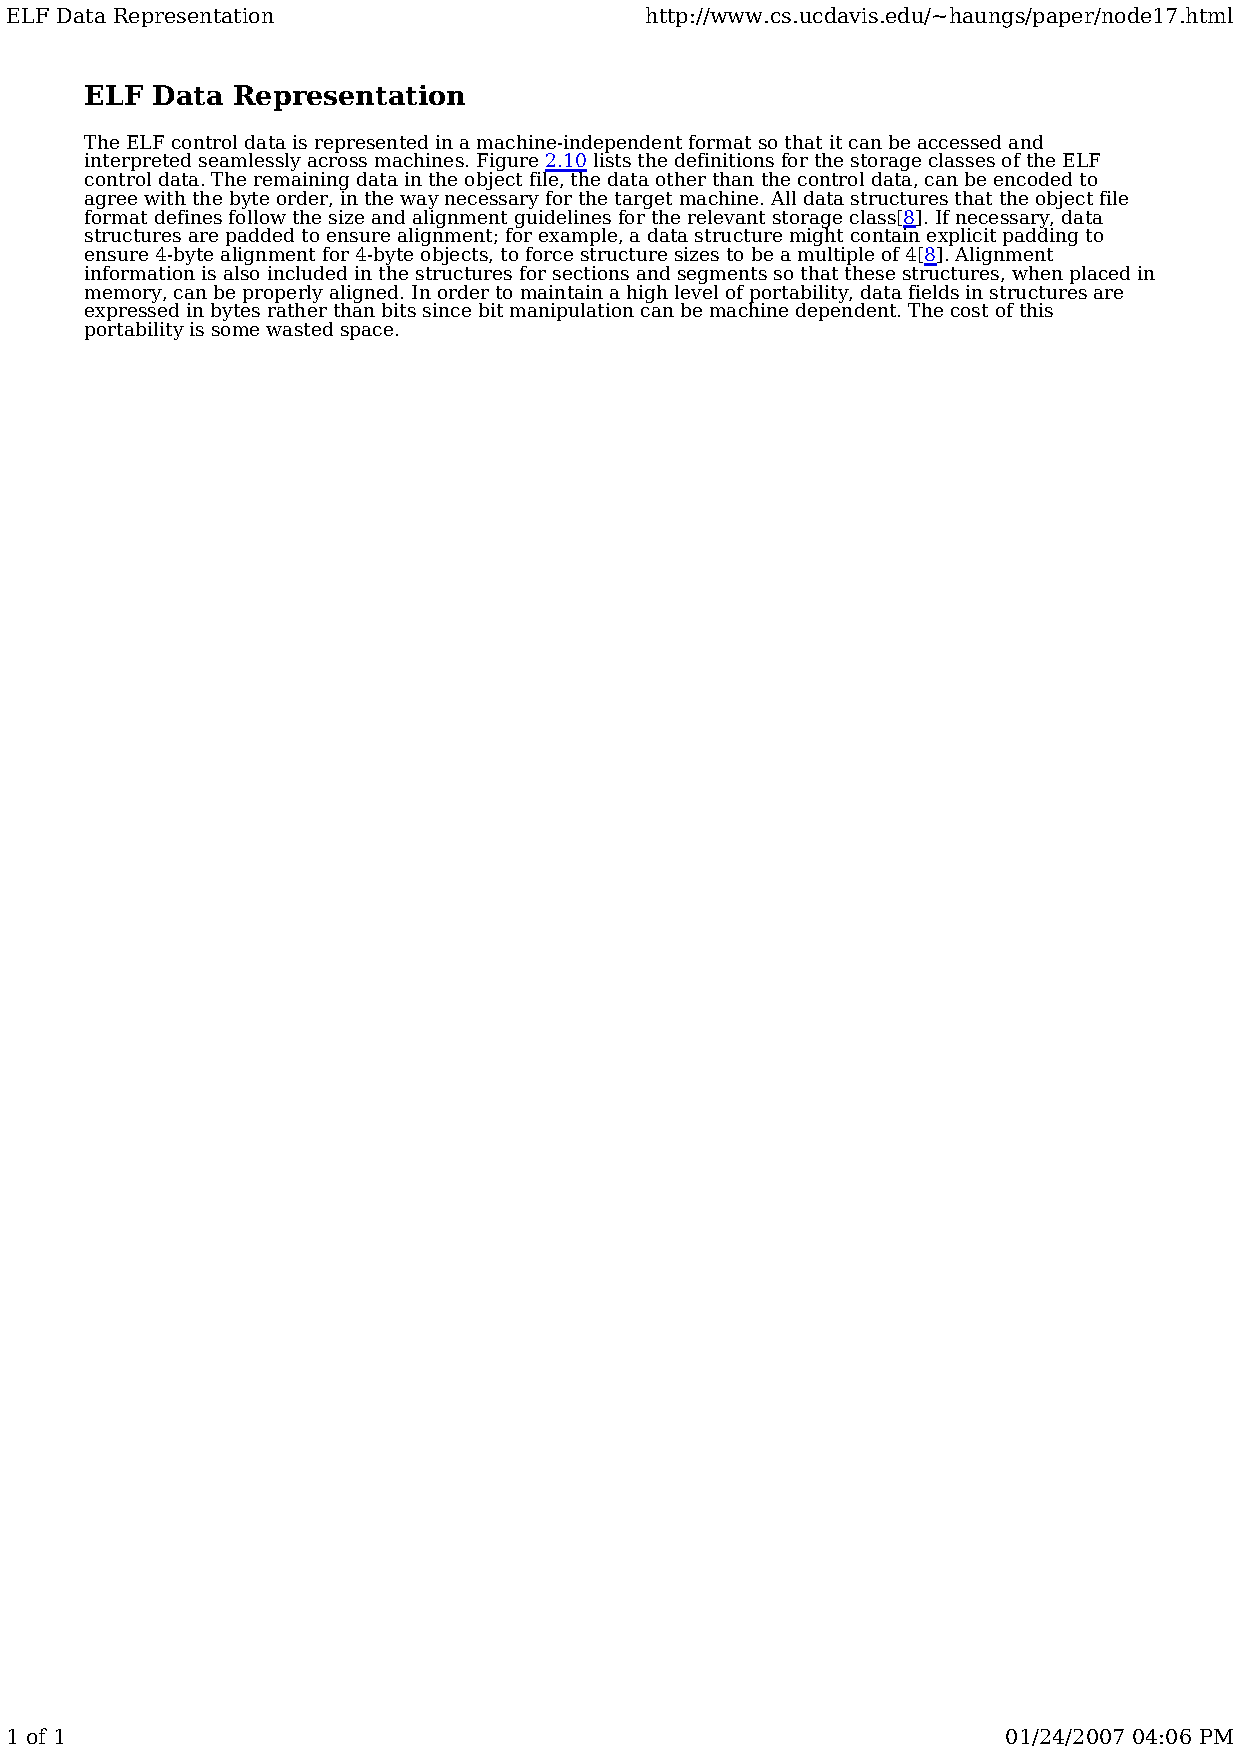
\includepdf[pages=-]{elf7}

%
% IA-32 operating mode switch
%

\section{IA-32 operating modes}

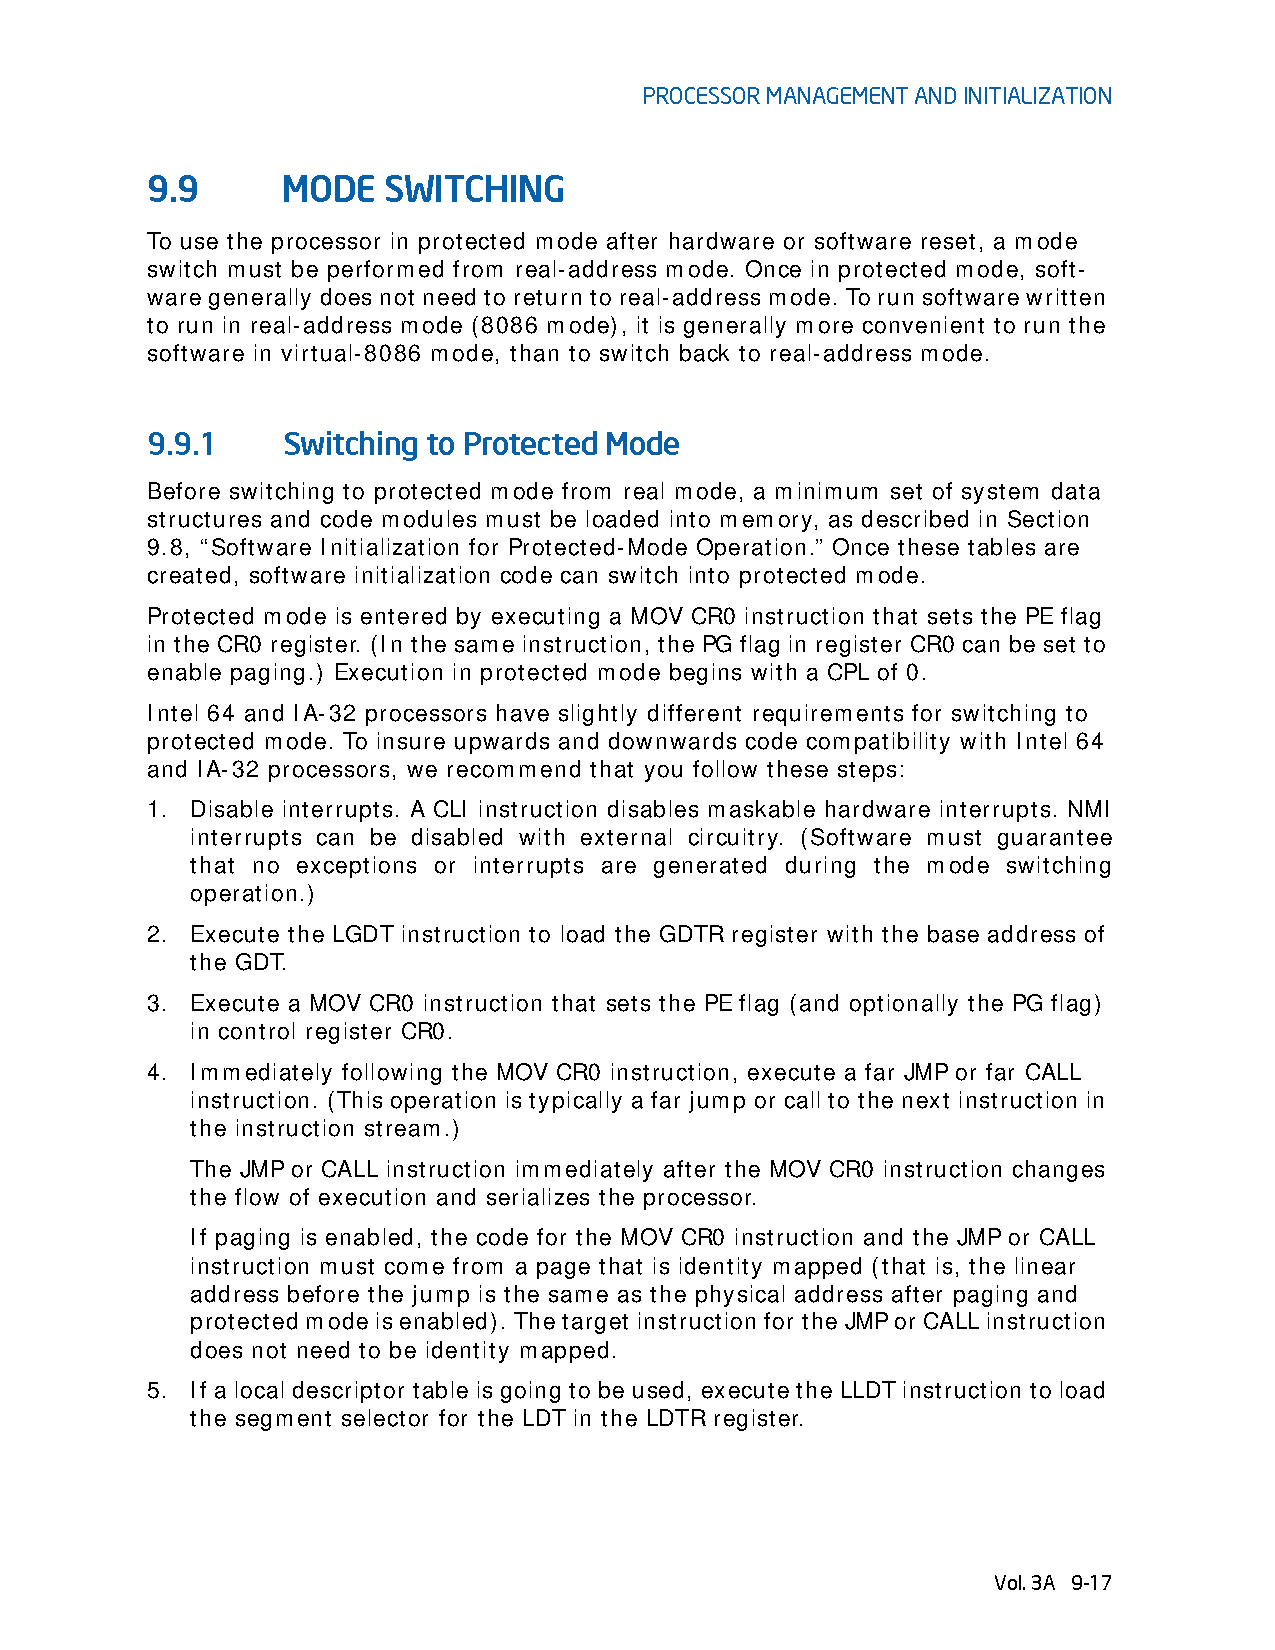
\includepdf[pages=-]{mode_switch}

\end{document}
